%% Manuscript converted to the Elsevier CAS single-column template (cas-sc.cls)
%% Base template: cas-sc-template.tex (Elsevier CAS Bundle v2.4)
\PassOptionsToPackage{hypertexnames=false}{hyperref}
\documentclass[a4paper,fleqn]{cas-sc}

% Numbered citation scheme (matches the numeric \cite style used throughout
% this manuscript and the existing thebibliography list below).
\usepackage[numbers,sort&compress]{natbib}

% --- Packages required by the manuscript content that are NOT already
% provided by cas-sc.cls (which already loads graphicx, amsmath, amsfonts,
% amssymb, booktabs, xcolor[svgnames,dvipsnames], hyperref, etc.) ---
\usepackage{algorithm}
\usepackage{algpseudocode}
\usepackage{float}
\usepackage{tikz}
\usetikzlibrary{shapes.geometric, arrows.meta, positioning, calc, fit}
% Use a scalable (outline) sans-serif font for the TikZ diagrams below,
% instead of the default Computer Modern Sans, which requires on-the-fly
% Metafont bitmap generation at arbitrary resized resolutions and can fail
% in TeX installations without a working Metafont mode setup.
\usepackage{helvet}
\usepackage{tabularx}
\usepackage{placeins}
\usepackage{siunitx}
\newcolumntype{C}{>{\centering\arraybackslash}X}
\newcolumntype{L}{>{\raggedright\arraybackslash}X}

% Relax float placement parameters to prevent queue congestion and avoid
% figures/tables drifting to the end of the document.
\renewcommand{\topfraction}{.9}
\renewcommand{\bottomfraction}{.8}
\renewcommand{\textfraction}{.07}
\renewcommand{\floatpagefraction}{.7}

% Align floats to the top of float-only pages instead of vertically centering them
\makeatletter
\setlength{\@fptop}{0pt}
\setlength{\@fpsep}{12pt}
\setlength{\@fpbot}{0pt plus 1fil}
\makeatother

\begin{document}
\let\WriteBookmarks\relax
\def\floatpagepagefraction{1}
\def\textpagefraction{.001}
%==========================================================
% Short Title
%==========================================================
\shorttitle{Grounded Neuro-Symbolic RAG for Semiconductor Device Physics}

%==========================================================
% Short Authors
%==========================================================
\shortauthors{Yalamarthi et al.}

%==========================================================
% Title
%==========================================================
\title[mode=title]{Verification-Guided Retrieval-Augmented Generation for Reliable Semiconductor Device Physics Reasoning}

%==========================================================
% Authors
%==========================================================

\author[1]{Yalamarthi Madhav}
\fnmark[1]
\ead{am.sc.u4aie23163@am.students.amrita.edu}
\credit{Conceptualization, Data curation, Methodology, Writing -- original draft, Writing -- review \& editing}

\author[1]{Ansh Bajpai}
\fnmark[1]
\ead{am.sc.u4aie23108@am.students.amrita.edu}
\credit{Methodology, Software, Validation, Investigation, Formal analysis}

\author[1]{Nishant Shah}
\fnmark[1]
\ead{am.sc.u4aie23166@am.students.amrita.edu}
\credit{Software, Investigation, Formal analysis, Writing -- review \& editing}

\author[1]{G Veena}
\cormark[1]
\credit{Conceptualization, Methodology, Supervision, Writing -- review \& editing}

\author[2]{Vani Kanjirangat}
\credit{Supervision, Methodology, Validation, Writing -- review \& editing}

%==========================================================
% Affiliations
%==========================================================

\affiliation[1]{organization={School of Computing, Amrita Vishwa Vidyapeetham},
city={Kollam},
state={Kerala},
country={India}}

\affiliation[2]{organization={SUPSI, IDSIA},
country={Switzerland}}

%==========================================================
% Footnotes
%==========================================================

\cortext[1]{Corresponding author.\\
E-mail: \texttt{veenag@am.amrita.edu}}

\fntext[1]{Yalamarthi Madhav, Ansh Bajpai, and Nishant Shah contributed equally to this work.}


% Here goes the abstract
\begin{abstract}
Although large language models can perform scientific reasoning, they often generate
incorrect equations, use variables inconsistently, or produce physically unrealistic values
because they rely on probability rather than physical laws. While retrieval-augmented
generation (RAG) helps ground responses in text, existing methods do not verify if generated
equations are mathematically and physically correct. To address this, our primary
contribution is a verification-centric RAG framework that explicitly enforces symbolic
and physical consistency before selecting the final answer. We implement this framework by
pairing a small, fine-tuned language model with a three-stage validation pipeline that
checks every generated equation by parsing it symbolically with SymPy, verifying its units
through dimensional analysis, and testing its numerical output against realistic parameters
across different semiconductor technology nodes. 
% To support generation, we use a hybrid
% retrieval system to extract governing equations from textbooks and inject them directly
% into the model's prompt. We evaluated our system on a benchmark of 100 semiconductor physics
% questions. On simple formula-recall questions, an ungrounded Llama-3.1-70B baseline performed
% better. However, on complex reasoning problems involving short-channel effects, our system
% achieved a physics validation score of 1.868 (on a custom 0--4 scale measuring equation
% correctness), compared to just 0.795 for the 70B baseline---a 135\% improvement
% (Wilcoxon $p = 0.002$, effect size $r = 0.677$, large effect). These results demonstrate
% that a small model constrained by physical rules can produce more reliable scientific
% formulas than a much larger model, suggesting that explicit validation may be more
% effective than parameter scaling for specialized physics tasks.
To improve the specified kind of output, a hybrid model is used which can extract equations from textbooks and import them directly into the prompt. The model was evaluated on a benchmark set of 100 semiconductor physics questions. For straightforward formula-recall questions, the model based on Llama-3.1-70B was found to demonstrate superior performance. However, for difficult reasoning questions on short-channel effects, the model achieved a physics validation score of $1.868$ for equation effectiveness from a scale of $0$ to $4$, while the Llama-3.1-70B-based model achieved only $0.795$ as a score and thus a differentiation of $135\%$ (Wilcoxon $p = 0.002$, effect size $r = 0.677$, which is considered large).
\end{abstract}

% Research highlights (3--5 bullets, each <= 85 characters)
\begin{highlights}
\item A three-stage SymPy pipeline checks equation syntax, dimensions, and values.
\item A 0.5B fine-tuned model with validation outperforms an ungrounded 70B model.
\item Physics score improves 135\% on hard questions vs.\ 70B baseline ($p=0.002$).
\item Verification-guided Best-of-N replaces stochastic sampling with a physics score.
\item Runs on a single 8GB laptop GPU, cutting VRAM use 116x vs.\ the cloud baseline.
\end{highlights}

% Keywords
\begin{keywords}
Neuro-Symbolic AI \sep Retrieval-Augmented Generation \sep Small Language Models \sep Semiconductor Device Physics \sep Equation Validation \sep Trustworthy AI
\end{keywords}

\maketitle

%%%%%%%%%%%%%%%%%%%%%%%%%%%%%%%%%%%%%%%%%%%%%%%%%%%%%%%%%%%%%%%%%%

\section{Introduction}
% Large Language Models (LLMs) have become widely used tools for answering questions, writing text, and helping with technical tasks across many different fields \citep{brown2020gpt3, touvron2023llama}, and researchers have naturally started exploring whether these models can also help with scientific and engineering work, such as answering domain-specific questions or generating technical content \citep{taylor2022galactica}. However, scientific reasoning presents unique challenges: LLMs frequently generate equations that look superficially correct but are dimensionally inconsistent, mathematically erroneous, or physically implausible \citep{PHYSICSEVAL-2024, Amrita-ScientificAI}. In fields like semiconductor device physics \citep{Sze-Book}, where even minor equation errors propagate into incorrect engineering designs, scaling model size alone does not resolve these failure modes \citep{ji2023survey,bang2023multitask}. This highlights a key research gap: current RAG architectures lack mechanisms to verify the symbolic correctness and physical consistency of generated formulas. To bridge this gap, we introduce a neuro-symbolic RAG framework that explicitly validates the dimensions and numerical limits of generated equations before final candidate selection.
Using Large Language Models (LLMs), it has become easy to write text, answer questions, and accomplish technical tasks across different fields \citep{brown2020gpt3, touvron2023llama}. As a result, researchers have expressed interest in using these models for scientific and engineering purposes, such as answering questions in specific domains and producing technical documentation \citep{taylor2022galactica}. Nevertheless, scientific reasoning introduces difficulties for LLMs, as they often produce equations that appear to be correct at first glance but are dimensionally inconsistent, mathematically wrong, or physically infeasible \citep{SciBench,INDUS2024}. For example, in semiconductor physics \citep{Sze-Book}, even a minor mistake in an equation can lead to an incorrect specification in engineering terms; thus, merely enlarging the model does not save the problem \citep{ji2023survey, bang2023multitask}. This highlights a key research gap: current RAG architectures lack mechanisms to verify the symbolic correctness and physical consistency of generated formulas. To bridge this gap, we introduce a neuro-symbolic RAG framework that explicitly validates the dimensions and numerical limits of generated equations before final candidate selection.

Retrieval-Augmented Generation (RAG) is one way to help with this. By fetching relevant documents at query time and using them to ground the model's response, RAG systems can improve factual accuracy and domain relevance \citep{RAG-Lewis, Gao-RAG-Survey}. That said, retrieval alone is not enough to guarantee that generated equations are physically valid. Even when a model has access to the right source material, it can still make mistakes like substituting the wrong variable or constructing an equation that does not hold up dimensionally. Many modern evaluation and verification frameworks rely on another language model as a judge to assess response quality \citep{zheng2023judging}. However, LLM-based judges suffer from stochastic inconsistency and position bias, and they frequently overlook subtle mathematical or physical errors \citep{zheng2023judging, SciBench}. For scientific applications, we need more reliable validation methods—specifically, deterministic checks based on mathematical rules, physical laws, and numerical range verification. Furthermore, relying on massive foundation models for scientific QA introduces significant computational overhead and cloud dependencies, limiting their viability for academic research, edge deployments, or privacy-sensitive applications. This underscores the need for lightweight architectures that can run locally on consumer-grade hardware while maintaining scientific reliability through external validation \citep{Qwen-Report, LoRA-Hu}.

To address these issues, we propose a lightweight neuro-symbolic verification system for retrieval-augmented generation (RAG) in semiconductor device physics. Central to our approach is a hypothesis-testing paradigm where each generated equation is treated as a candidate hypothesis that must survive three independent, complementary physical validation checks before being accepted as trustworthy. Specifically, the pipeline couples a small, fine-tuned language model with hybrid retrieval and a three-stage deterministic validation layer consisting of: (1) symbolic parsing with SymPy, (2) coverage-aware dimensional analysis, and (3) multi-node numerical plausibility testing. The key idea is that a small model, when given the right retrieved context and constrained by deterministic physics checks, can produce more reliable scientific answers than a larger model relying purely on memorized knowledge. Our specific contributions include:
\begin{itemize}
\item We propose a deterministic verification framework for scientific RAG that validates generated equations through symbolic parsing, dimensional consistency analysis, and numerical plausibility testing before accepting generated responses.
\item We introduce a verification-guided Best-of-N candidate selection strategy that replaces stochastic sampling with a physics-score-driven argmax over multiple generated candidates.
\item We show that, on complex multi-step reasoning questions, retrieval grounding combined with symbolic verification enables a sub-billion-parameter model to produce more physically consistent equations than a substantially larger ungrounded model, indicating that explicit validation can be a more effective lever than parameter scaling for this class of problem.
\item We present a practical neuro-symbolic RAG architecture for semiconductor device physics that is domain-agnostic at its verification core, allowing the retrieval corpus and physical-dimension/parameter mappings to be swapped to generalize the framework to other equation-governed scientific domains.
\end{itemize}

%%%%%%%%%%%%%%%%%%%%%%%%%%%%%%%%%%%%%%%%%%%%%%%%%%%%%%%%%%%%%%%%%%
\section{Related Work}
Scientific question answering and equation generation are active areas of research. This section briefly reviews prior work on retrieval-augmented generation in science, efficient fine-tuning of small models, evaluation methods for scientific AI, and neuro-symbolic approaches.

\subsection{Retrieval-Augmented Generation in Scientific Domains}
RAG was introduced by Lewis et al.\ \citep{RAG-Lewis} as a way to give language models access to external knowledge at inference time. Dense retrieval methods like DPR \citep{DPR-Karpukhin} further showed that embedding-based passage retrieval can outperform traditional keyword search for open-domain question answering. In scientific settings, RAG has been used to retrieve formulas, explanations, and reference material from textbooks and papers, including applications in medical \citep{Amrita-RAG-Medical} and engineering domains \citep{Engineering-RAG, Amrita-Vinayakumar-2018}. Evaluation tools like RAGAS \citep{RAGAS-Es} and ARES \citep{ARES-ACL} measure how well a RAG system retrieves and uses relevant content, but these tools mostly focus on text overlap and semantic similarity—they do not check whether a generated equation is dimensionally consistent or numerically correct. A response can be rated highly by these metrics while still containing a wrong equation. Our work adds a symbolic verification layer on top of retrieval to catch exactly these kinds of errors, instead of treating generated equations as plain text.

\subsection{Lightweight Language Models and Efficient Fine-Tuning}
Deploying large models in reality needs substantial computer resources, which thereby creates worries regarding the cost and security of information. Parameter-Efficient Fine-Tuning (PEFT) methods, particularly Low-Rank Adaptation (LoRA) \citep{LoRA-Hu}, allow compact models like Qwen2.5 \citep{Qwen-Report} to specialize in narrow scientific domains by training low-rank adapter matrices rather than updating all model weights. Small language models do well on domain-specific vocabulary after fine-tuning, but they tend to struggle with zero-shot mathematical reasoning and are more prone to hallucinating formulas. Our approach tries to compensate for this by adding retrieval grounding and a deterministic verification step so that the model’s weaker reasoning is guided and checked rather than left unconstrained. Similar dataset curation and modeling efforts have been explored for domain-specific text classification tasks \citep{Amrita-Naveenkumar-2020}.

\subsection{Evaluation Frameworks for Scientific AI Systems}
Typically, standard language model evaluations focus on the fluency and semantic quality of generated text rather than the correctness of underlying scientific reasoning. Although scientific reasoning benchmarks such as SciBench~\citep{SciBench} assess scientific problem-solving capabilities, they do not explicitly verify equation correctness, dimensional consistency, or adherence to semiconductor device physics. do exist; they usually utilize a large language model to determine whether an answer is valid. The problem with the "LLM-as-a-judge" strategy is that this practice can end up being inconsistent and might overlook some mistakes in mathematical equations \citep{Ali2023XAI}. To resolve validation challenges in specialized text processing, deep learning models coupled with Explainable AI (XAI) techniques have been successfully applied to domain-specific text classification and verification problems \citep{Amrita-Likha-2025}. Scientific knowledge grounding conducted with the help of domain-specific systems has proven that standard text evaluation does not allow us to understand if the answers given by a model are correct from the physics and math point of view \citep{INDUS2024}. In this paper, we explore another way and propose a validation pipeline that uses SymPy and performs symbolic analysis, dimensional analysis, and checking the range of numerical values, providing unconditional, reproducible results that do not require any external model.

\subsection{Neuro-Symbolic AI and Deterministic Scientific Validation}
Neuro-symbolic AI refers to the combination of learned neural representations with rule-based symbolic reasoning \citep{Garcez-NeuroSymbolic, XAI-Barredo}. Most of the existing neuro-symbolic systems focus on structured inputs or predefined logic graphs, and they are not meant for handling the types of free-form text that the LLMs generate. Recent literature has shown interest in using neuro-symbolic validation as a manner of making the AI outputs trustworthy in engineering applications \citep{Gaur2024}, and hybrid retriever setups have also been studied \citep{Doan2024Hybrid}. Our validation layer makes a step toward achieving this goal by translating the generated equations into symbolic expressions and applying the predetermined laws of physics instead of considering them to be just text strings. Similar deep feature learning methods with evolutionary optimization have been explored for specialized engineering domains \citep{Amrita-Anand-2026}.

Despite progress in both RAG systems and neuro-symbolic AI, a clear gap remains: existing RAG pipelines for scientific domains lack built-in mechanisms to verify the physical and mathematical correctness of generated equations. Text-similarity metrics such as BLEU, ROUGE, and BERTScore, as well as LLM-as-a-judge evaluation, are insufficient for catching dimensional errors or numerically implausible results. At the same time, neuro-symbolic approaches have not yet been adapted to free-form scientific text generation in resource-constrained settings. There is also little prior work that validates generated equations across multiple semiconductor technology nodes or that studies how best-of-$n$ candidate selection interacts with physics-based scoring. This work directly addresses these gaps by combining hybrid retrieval, equation-grounded prompting, and a deterministic three-step validation pipeline within a sub-billion-parameter model that can run on a single consumer GPU.

%%%%%%%%%%%%%%%%%%%%%%%%%%%%%%%%%%%%%%%%%%%%%%%%%%%%%%%%%%%%%%%%%%

\section{Proposed Methodology}
The proposed methodology combines hybrid retrieval, equation-grounded prompting, and our three-stage neuro-symbolic verification system to produce physically and mathematically coherent responses from a tiny language model. Our methodology is organised as a decoupled pipeline that keeps deterministic physical verification and probabilistic language production apart.  The overall architecture is shown in Figure~\ref{fig:architecture}.

We formalize the execution flow of the proposed neuro-symbolic verification framework as a sequential decision and validation pipeline. To facilitate readability, the mathematical symbols and notations used throughout this manuscript are summarized in Table~\ref{tab:notations}.
\begin{figure}[pos=tp] 
\centering
\resizebox{0.95\linewidth}{!}{%
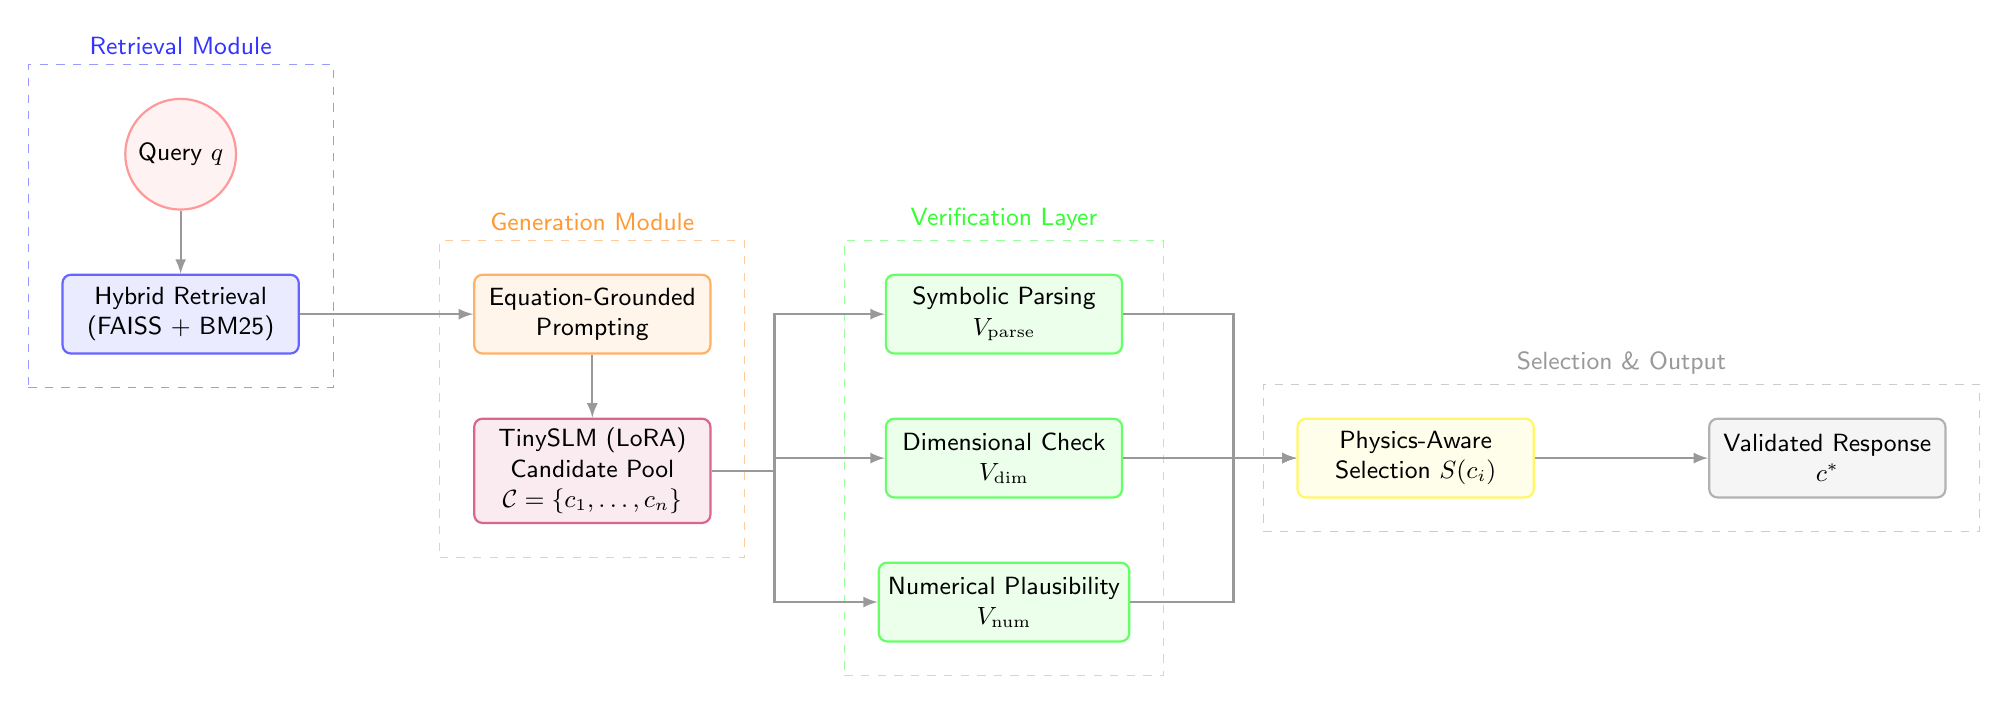
\begin{tikzpicture}[
    font=\sffamily\small,
    node distance=0.8cm and 2.2cm,
    box/.style={draw, rectangle, rounded corners=3pt, minimum width=3.0cm, minimum height=1.0cm, align=center, fill=white, draw=gray!80, thick},
    retrieval/.style={box, fill=blue!8, draw=blue!60},
    prompt/.style={box, fill=orange!8, draw=orange!60},
    generation/.style={box, fill=purple!8, draw=purple!60},
    validation/.style={box, fill=green!8, draw=green!60},
    selection/.style={box, fill=yellow!8, draw=yellow!60},
    input/.style={box, fill=red!5, draw=red!40, circle, minimum width=1.2cm},
    output/.style={box, fill=gray!8, draw=gray!60},
    arrow/.style={-latex, thick, draw=gray!80},
    dasharrow/.style={-latex, dashed, thick, draw=gray!60},
    labelstyle/.style={font=\sffamily\scriptsize\bfseries}
]

% Column 1: Ingestion & Retrieval
\node[input] (query) {Query $q$};
\node[retrieval, below=0.8cm of query] (hybrid) {Hybrid Retrieval\\(FAISS + BM25)};

% Column 2: Prompting & SLM Candidate Generation
\node[prompt, right=2.2cm of hybrid] (prompt) {Equation-Grounded\\Prompting};
\node[generation, below=0.8cm of prompt] (generation) {TinySLM (LoRA)\\Candidate Pool\\$\mathcal{C} = \{c_1, \dots, c_n\}$};

% Column 3: Verification Gauntlet (Vertical Stack)
\node[validation, right=2.2cm of prompt] (val_parse) {Symbolic Parsing\\$V_{\mathrm{parse}}$};
\node[validation, below=0.8cm of val_parse] (val_dim) {Dimensional Check\\$V_{\mathrm{dim}}$};
\node[validation, below=0.8cm of val_dim] (val_num) {Numerical Plausibility\\$V_{\mathrm{num}}$};

% Column 4: Selection & Output
\node[selection, right=2.2cm of val_dim] (selection) {Physics-Aware\\Selection $S(c_i)$};
\node[output, right=2.2cm of selection] (final) {Validated Response\\$c^*$};

% Group Frames
\node[draw=blue!40, dashed, inner sep=12pt, fit=(query) (hybrid), label={[text=blue!80]above:Retrieval Module}] (g1) {};
\node[draw=orange!40, dashed, inner sep=12pt, fit=(prompt) (generation), label={[text=orange!80]above:Generation Module}] (g2) {};
\node[draw=green!40, dashed, inner sep=12pt, fit=(val_parse) (val_dim) (val_num), label={[text=green!80]above:Verification Layer}] (g4) {};
\node[draw=gray!40, dashed, inner sep=12pt, fit=(selection) (final), label={[text=gray!80]above:Selection \& Output}] (g5) {};

% Connections
\draw[arrow] (query) -- (hybrid);
\draw[arrow] (hybrid) -- (prompt);
\draw[arrow] (prompt) -- (generation);
\draw[arrow] (generation.east) -- ++(0.8,0) |- (val_parse.west);
\draw[arrow] (generation.east) -- ++(0.8,0) |- (val_dim.west);
\draw[arrow] (generation.east) -- ++(0.8,0) |- (val_num.west);

\draw[arrow] (val_parse.east) -| ($(selection.west)-(0.8,0)$) -- (selection.west);
\draw[arrow] (val_dim.east) -- (selection.west);
\draw[arrow] (val_num.east) -| ($(selection.west)-(0.8,0)$) -- (selection.west);
\draw[arrow] (selection) -- (final);

\end{tikzpicture}%
}
\caption{Overall architecture of the proposed verification-guided retrieval-augmented generation framework. The pipeline combines hybrid retrieval, equation-aware prompting, multi-candidate generation, deterministic symbolic verification, and physics-guided candidate selection.}
\label{fig:architecture}
\end{figure}
\begin{table}[!t]
\caption{Summary of mathematical notation and symbols used in the neuro-symbolic retrieval-augmented generation (RAG) framework, including evaluation parameters, decision routing variables, and right-hand side (RHS) symbol definitions.}
\label{tab:notations}
\centering
\begin{tabularx}{\linewidth}{@{}lX@{}}
\toprule
\textbf{Symbol} & \textbf{Description} \\
\midrule
$q$ & User query or physics question \\
$\mathcal{E}$ & Concatenated retrieved evidence chunks \\
$E_q$ & Governing physical equation extracted from the corpus chunks \\
$P(q, E_q)$ & Equation-grounded prompt \\
$\mathcal{C}$ & Set of generated candidate responses $\{c_1, c_2, \dots, c_n\}$ \\
$c_i$ & A single generated candidate response \\
$c^*$ & Selected optimal candidate response \\
$\theta$ & Parameter weights of the adapted small language model (SLM) \\
$p_\theta$ & Candidate generation probability distribution of the SLM \\
$S_{\mathrm{phys}}(c_i)$ & Programmatic physics validation score of candidate $c_i$ \\
$S_{\mathrm{sim}}(c_i, \mathcal{E})$ & Semantic cosine similarity between candidate $c_i$ and evidence $\mathcal{E}$ \\
$\mathcal{S}(c_i)$ & Selection objective score of candidate $c_i$ \\
$\alpha$ & Regularization parameter for semantic tie-breaking ($10^{-4}$) \\
$V_{\mathrm{parse}}(c_i)$ & Symbolic parseability indicator ($\in \{0,1\}$) \\
$V_{\mathrm{dim}}(c_i)$ & Dimensional consistency indicator ($\in \{0,1\}$) \\
$V_{\mathrm{num}}(c_i)$ & Numerical plausibility indicator ($\in \{0,1\}$) \\
$f_{\mathrm{cov}}(c_i)$ & RHS symbol vocabulary coverage fraction ($\in [0,1]$) \\
\tau_{\mathrm{dim}} & Symbol coverage threshold for dimensional check ($0.70$) \\
$C(c_i)$ & Comprehensive confidence score ($\in [0,1]$) \\
$w_j$ & Weight parameters for the confidence score components \\
$m_{\mathrm{route}}$ & Routing mode of the query, $m_{\mathrm{route}} \in \{\text{Lookup}, \text{Explore}, \text{Sweep}\}$ \\
\bottomrule
\end{tabularx}
\end{table}

Given an input query $q$, the orchestrator first determines the query routing mode $m_{\mathrm{route}} \in \{\text{Lookup}, \text{Explore}, \text{Sweep}\}$: Lookup routes simple factual queries directly to the retrieval engine for a corpus-grounded answer without equation generation. Explore routes analytical queries that require the model to generate and justify a governing equation for a specific scenario, and sweep routes parametric queries that require evaluating a governing equation across a range of parameter values or technology nodes (e.g., plotting a quantity such as $g_m$ versus $I_d$).

For analytical queries requiring equation generation ($m_{\mathrm{route}} \in \{\text{Explore}, \text{Sweep}\}$), the pipeline proceeds through three stages: grounded retrieval, candidate generation, and symbolic verification. First, a hybrid retrieval engine searches the document corpus to extract relevant chunks $D_q$. These chunks are parsed to isolate governing physical equations $E_q$ (using the extraction and normalization procedures detailed in Section~\ref{subsec:equation_extraction}), which are then prepended to the user query to construct an equation-grounded prompt $P(q, E_q)$.

Second, the domain-adapted small language model (parameterized by $\theta$) is used to generate a set of $n$ independent candidate responses:
\begin{equation*}
\mathcal{C} = \{c_1, c_2, \dots, c_n\} \quad \text{where} \quad c_i \sim p_{\theta}(c \mid P(q, E_q))
\end{equation*}

Third, each candidate response $c_i$ is processed by our verification layer, which identifies and extracts mathematical equations $e \in c_i$ (as detailed in Section~\ref{subsec:equation_extraction}). Each equation is subjected to a three-stage verification pipeline: symbolic parsing via SymPy, algebraic dimensional analysis, and multi-node numerical range checks. Finally, these validation signals are aggregated with retrieval features to select the optimal candidate $c^*$ that maximizes a selection objective score $\mathcal{S}(c_i)$:
\begin{equation*}
c^* = \operatorname*{arg\,max}_{c_i \in \mathcal{C}} \mathcal{S}(c_i)
\end{equation*}
as the final response, where the selection score $\mathcal{S}(c_i)$ integrates the physics validation score and semantic relevance as formulated in Section~\ref{subsec:selection}.

\subsection{Hybrid Retrieval Subsystem}
\label{subsec:retrieval}
The retrieval module augments the parametric knowledge of the SLM with domain-specific evidence. The dense path uses FAISS \citep{FAISS-Johnson} with \texttt{bge-large-en-v1.5} embeddings \citep{BGE-Xiao} to find semantically similar chunks. The semiconductor corpus---described in detail in Section~\ref{subsec:doc_corpora}---is divided into physics-aware chunks while preserving equation structure. Building and training structured grammars and lexical databases over large-scale textbook corpora can also leverage parallelized computational frameworks, such as MapReduce and Spark workflows \citep{Amrita-Author-2016}. The sparse path uses BM25 \citep{BM25-Robertson}, augmented with a custom, physics-aware regular expression tokenizer that we proposed and designed specifically for this work. The tokenizer is defined by the regular expression pattern:
\begin{equation*}
\mathcal{P} = \verb|[A-Za-z][A-Za-z0-9_]*| \;\cup\; \verb|\d+(?:\.\d+)?(?:[eE][+-]?\d+)?|
\end{equation*}
The first branch matches alphanumeric variables (e.g., physics symbols), while the second branch matches numbers (including floating-point and scientific notation constants), discarding mathematical operator noise.

To illustrate the necessity of this custom tokenizer, consider the expression \texttt{(Vgs-Vth)\textsuperscript{2}} alongside the physical constant charge value \texttt{1.6e-19}:
\begin{itemize}
    \item A \textbf{standard whitespace tokenizer} splits solely on spaces, yielding the single atomic tokens \texttt{["(Vgs-Vth)\textsuperscript{2}"]} and \texttt{["1.6e-19"]}. Consequently, a user query containing \texttt{Vth} fails to match this document chunk because the sub-string is bound inside the equation token.
    \item A \textbf{standard alphanumeric/punctuation tokenizer} (splitting on non-word characters) splits the equation into \texttt{["Vgs", "Vth", "2"]}, but breaks the scientific constant into fragmented tokens: \texttt{["1", "6", "e", "19"]}, destroying the constant's semantic meaning.
    \item Our \textbf{proposed physics-aware tokenizer} extracts the exact set of physical symbols and constants as atomic units, yielding \texttt{["Vgs", "Vth"]} and \texttt{["1.6e-19"]}. This simultaneously preserves the integrity of scientific constants while exposing internal equation symbols (\texttt{Vgs}, \texttt{Vth}) to sparse index search queries.
\end{itemize}
The two ranked lists are combined using Reciprocal Rank Fusion (RRF) \citep{RRF-Cormack}:
\begin{equation*}
\mathrm{Score}_{\mathrm{RRF}}(d \in D) = \sum_{m \in M} \frac{1}{k + r_m(d)}
\end{equation*}
where $r_m(d)$ is the rank of the document chunk $d$ under the retrieval method $m$, and $k$ is a smoothing constant. After fusion, a cross-encoder using \texttt{ms-marco-MiniLM-L-6-v2} reranks the top candidates. The highest-ranked chunks are then scanned using a heuristic-based equation detector---distinct from the SymPy-based symbolic parser used later for candidate verification (Section~\ref{subsec:equation_extraction})---which flags equation-like spans via pattern cues such as explicit equality symbols and recognized device-physics notation, while rejecting non-equation text (e.g., stray symbol sequences) using the same letter-soup rejection criterion described in Section~\ref{subsec:equation_extraction}. The system finds the most accurate equation from the retrieved textbooks and adds it directly to the prompt. This gives the model clear physical equations to use as evidence while generating its answer. The full process of combining this search with equation extraction—along with a real-world example—is illustrated in Figure~\ref{fig:retrieval_workflow}.

\begin{figure}[pos=tp] 
\centering
\resizebox{\linewidth}{!}{%
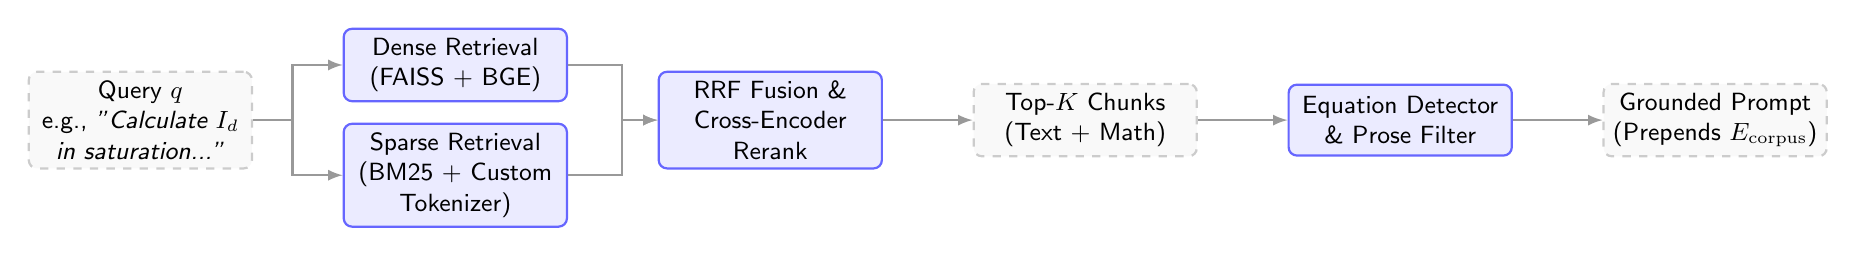
\begin{tikzpicture}[
    font=\sffamily\small,
    box/.style={draw, rectangle, rounded corners=3pt, text width=2.6cm, minimum height=0.9cm, align=center, fill=white, draw=gray!80, thick},
    stepbox/.style={box, fill=blue!8, draw=blue!60},
    databox/.style={box, fill=gray!5, draw=gray!40, dashed},
    arrow/.style={-latex, thick, draw=gray!80},
    labelstyle/.style={font=\sffamily\scriptsize\bfseries}
]

% Column 1: Input Query
\node[databox] (query) at (0,0) {Query $q$\\e.g., \textit{"Calculate $I_d$ in saturation..."}};

% Column 2: Parallel Retrieval Paths
\node[stepbox] (dense) at (4.0, 0.7) {Dense Retrieval\\(FAISS + BGE)};
\node[stepbox] (sparse) at (4.0,-0.7) {Sparse Retrieval\\(BM25 + Custom Tokenizer)};

% Column 3: Fusion & Rerank
\node[stepbox] (rrf) at (8.0, 0) {RRF Fusion \&\\Cross-Encoder Rerank};

% Column 4: Top Candidates
\node[databox] (chunks) at (12.0, 0) {Top-$K$ Chunks\\(Text + Math)};

% Column 5: Equation Detector
\node[stepbox] (detector) at (16.0, 0) {Equation Detector\\\& Prose Filter};

% Column 6: Grounded Prompt
\node[databox] (output) at (20.0, 0) {Grounded Prompt\\(Prepends $E_{\mathrm{corpus}}$)};

% Connections
\draw[arrow] (query.east) -- ++(0.5,0) |- (dense.west);
\draw[arrow] (query.east) -- ++(0.5,0) |- (sparse.west);
\draw[arrow] (dense.east) -| ($(rrf.west)-(0.45,0)$) -- (rrf.west);
\draw[arrow] (sparse.east) -| ($(rrf.west)-(0.45,0)$) -- (rrf.west);
\draw[arrow] (rrf) -- (chunks);
\draw[arrow] (chunks) -- (detector);
\draw[arrow] (detector) -- (output);

\end{tikzpicture}%
}
\caption{Workflow of the hybrid retrieval and in-context equation extraction subsystem, demonstrating how raw user queries are grounded with parsed equations using dense vector search (FAISS), keyword search (BM25), reciprocal rank fusion (RRF), and cross-encoder rerankers.}
\label{fig:retrieval_workflow}
\end{figure}

\subsection{Language Model Selection}
Using a compact model with less than one billion parameters, we can evaluate the effectiveness of our verification system under rigorous resource conditions. This indicates that the enhancements in performance are attributed to the verification mechanism rather than the size of the language model. For the purpose of this study, we opted for using \texttt{Qwen2.5-0.5B-Instruct} \citep{Qwen-Report} as a base model. While other sub-billion and low-parameter models exist (such as \texttt{TinyLlama-1.1B} \citep{zhang2024tiny} or \texttt{Llama-3.2-1B} \citep{dubey2024llama}), we explicitly choose the Qwen2.5 architecture because comparative benchmarks show that it significantly outperforms other small models on mathematical reasoning (e.g., GSM8K, MATH) and coding tasks \citep{Qwen-Report}. This capability of pre-trained model is crucial for generating structured mathematical equations and following precise LaTeX formatting constraints under highly restricted computational budgets.

\subsection{Deterministic Neuro-Symbolic Validation Pipeline}
It has been suggested that a deterministic verification system based on neuro-symbolic methods be employed to check the validity of equations produced by neuro-symbolic methods. Each response produced by the system is analyzed for mathematics involved in its production, and it is compared to deterministic principles of physics. The verification logic is formalized in Algorithm~\ref{alg:verification}. The verification system assesses the complementary features of the generated equations from syntactic relations to physical consistency.

\begin{algorithm}
\caption{Execution steps for the deterministic neuro-symbolic equation verification algorithm, outlining symbolic parsing, coverage-aware dimensional analysis, and node-specific numerical plausibility checks.}
\label{alg:verification}
\begin{algorithmic}[1]
\Require Candidate response text $T$, base dimension map $\mathcal{D}$, node profiles $\mathcal{P} = \{P_1, P_2, P_3\}$
\Ensure Verification scores $S_{\mathrm{sym}}, S_{\mathrm{dim}}, S_{\mathrm{num}}, S_{\mathrm{cov}} \in \{0, 1\}$
\State $E \leftarrow \text{ExtractEquations}(T)$
\If{$E = \emptyset$}
    \State $S_{\mathrm{sym}}, S_{\mathrm{dim}}, S_{\mathrm{num}}, S_{\mathrm{cov}} \leftarrow 0, 0, 0, 0$
    \State \Return $S_{\mathrm{sym}}, S_{\mathrm{dim}}, S_{\mathrm{num}}, S_{\mathrm{cov}}$
\EndIf
\For{each equation $e \in E$}
    \State $e_{\text{norm}} \leftarrow \text{NormalizeLaTeX}(e)$
    \State $(LHS, RHS) \leftarrow \text{SymPyParse}(e_{\text{norm}})$ \Comment{may raise \textbf{ParsingError}}
    \If{parsing succeeded}
        \State $S_{\mathrm{sym}} \leftarrow 1$
    \Else
        \State $S_{\mathrm{sym}} \leftarrow 0$
        \State \Return $S_{\mathrm{sym}}, S_{\mathrm{dim}}, S_{\mathrm{num}}, S_{\mathrm{cov}} \leftarrow 0, 0, 0, 0$
    \EndIf

    \State $symbols \leftarrow \text{ExtractSymbols}(LHS \cup RHS)$
    \State $recognized\_symbols \leftarrow \{s \in symbols \mid s \in \mathcal{D}\}$
    \If{$|recognized\_symbols| / |symbols| \geq 0.70$}
        \State $S_{\mathrm{cov}} \leftarrow 1$
    \Else
        \State $S_{\mathrm{cov}} \leftarrow 0$
    \EndIf

    \If{$S_{\mathrm{cov}} = 1$}
        \State $dim_{LHS} \leftarrow \text{ReduceDimensions}(LHS, \mathcal{D})$
        \State $dim_{RHS} \leftarrow \text{ReduceDimensions}(RHS, \mathcal{D})$
        \If{$dim_{LHS} \equiv dim_{RHS}$}
            \State $S_{\mathrm{dim}} \leftarrow 1$
        \Else
            \State $S_{\mathrm{dim}} \leftarrow 0$
        \EndIf
    \Else
        \State $S_{\mathrm{dim}} \leftarrow 0$
    \EndIf

    \State $passes \leftarrow 0$
    \For{each node profile $P \in \mathcal{P}$}
        \State $val_{LHS} \leftarrow \text{Evaluate}(LHS, P)$
        \State $val_{RHS} \leftarrow \text{Evaluate}(RHS, P)$ \Comment{on \textbf{EvaluationError}: skip this profile}
        \If{$\neg\,\text{IsNaNOrInf}(val_{LHS}, val_{RHS})$ \textbf{and} $\text{PhysicalRangeCheck}(val_{LHS}, val_{RHS})$}
            \State $passes \leftarrow passes + 1$
        \EndIf
    \EndFor
    \If{$passes \geq 2$}
        \State $S_{\mathrm{num}} \leftarrow 1$
    \Else
        \State $S_{\mathrm{num}} \leftarrow 0$
    \EndIf
\EndFor
\State \Return $S_{\mathrm{sym}}, S_{\mathrm{dim}}, S_{\mathrm{num}}, S_{\mathrm{cov}}$
\end{algorithmic}
\end{algorithm}

\subsubsection{Symbolic Equation Parsing}
\label{subsec:equation_extraction}
The first stage of the validation pipeline extracts and tokenizes mathematical relationships from the free-form text. The system scans the generated text using regular expressions to locate equations enclosed in LaTeX delimiters (e.g., \verb|$$...$$| or \verb|$...$|), or lines containing explicit equality symbols ($=$).

Once located, the equation string undergoes a multi-step normalization process to strip rendering syntax and map it to algebraic tokens. This includes translating fractional structures
(e.g., mapping \verb|\frac{a}{b}| to \verb|(a)/(b)|), converting multiplication indicators
(such as \verb|\cdot| or \verb|\times| to \verb|*|), and stripping LaTeX formatting keywords
(like \verb|\text|, \verb|\mathrm|, or styling braces). Subscripts (e.g., $C_{ox}$ or $V_{gs}$)
are normalized into contiguous alphabetical tokens (such as \texttt{Cox} or \texttt{Vgs}) to
ensure they are treated as unified variables rather than separate multiplication terms.

Finally, the normalized string is split by the equality symbol into left-hand side (LHS) and
right-hand side (RHS) substrings. These substrings are parsed into mathematical expression trees via SymPy's parsing library \citep{sympy}. This step checks syntactic validity by compiling the expressions into Abstract Syntax Trees (ASTs) composed of operation nodes (e.g., \texttt{Add}, \texttt{Mul},
\texttt{Pow}) and leaf nodes (\texttt{Symbol}, \texttt{Float}). Any equation that contains
invalid syntax, mismatched parentheses, or uninterpretable symbols fails to compile and is
immediately rejected.

\subsubsection{Coverage-Aware Dimensional Analysis}
Each symbol in the parsed equation is looked up in a dictionary that maps variable names to base physical dimensions: $[I, V, L, T, K, C]$ representing current, voltage, length, time, temperature, and charge, respectively. To evaluate the cumulative dimensions of each expression, the system performs a recursive post-order traversal over the SymPy Abstract Syntax Tree (AST) representing the equation's left-hand side (LHS) and right-hand side (RHS). The checker reduces the AST by evaluating each node according to its class:
\begin{itemize}
    \item \textbf{Symbol Nodes (\texttt{sp.Symbol}):} Resolves to the base dimension dictionary mapped to the variable name; if the symbol is unrecognized, it defaults to a dimensionless state ($\emptyset$).
    \item \textbf{Constant \& Function Nodes:} Predefined numerical constants (integers, floats, fractions) and transcendental functions (e.g., $\log$, $\ln$, $\exp$) evaluate directly to dimensionless ($\emptyset$).
    \item \textbf{Multiplication Nodes (\texttt{sp.Mul}):} Evaluates all child nodes and combines their dimensions by adding the corresponding exponents of their base dimensions (e.g., multiplying mobility $[L^2 V^{-1} T^{-1}]$ and capacitance $[I^1 T^1 V^{-1} L^{-2}]$ sums their exponents).
    \item \textbf{Power Nodes (\texttt{sp.Pow}):} Evaluates the base node's dimensions and scales its exponents by the float value of the exponent (e.g., a square root operation $\sqrt{x}$ is parsed as $x^{0.5}$, scaling all exponents of $\text{Dim}(x)$ by $0.5$).
    \item \textbf{Addition Nodes (\texttt{sp.Add}):} Evaluates all addends and verifies that they have identical dimensions ($\text{Dim}(a_i) \equiv \text{Dim}(a_j) \; \forall i, j$). If a mismatch is detected, a dimensional error is immediately raised and propagated.
\end{itemize}
An equation passes this check only if the simplified LHS and RHS dimension dictionaries are strictly equivalent:
\begin{equation*}
\mathrm{dims}_{\mathrm{LHS}}^{\{I,V,L,T,K,C\}}
\equiv
\mathrm{dims}_{\mathrm{RHS}}^{\{I,V,L,T,K,C\}}
\end{equation*}
This dimensional check is gated on a symbol coverage threshold of $\tau_{\mathrm{dim}} = 0.70$. This threshold was empirically calibrated to resolve a fundamental trade-off in automated dimensional checking:
\begin{itemize}
    \item If the threshold is set too low (e.g., $<0.50$), the engine runs on equations where the majority of variables are unrecognized and treated as dimensionless ($\emptyset$) by default. This leads to vacuous matches or false failures due to missing physical metadata.
    \item If the threshold is set too high (e.g., requiring $1.00$ coverage), any correct equation that introduces even a single unregistered helper variable, generic scaling coefficient (e.g., $A, B$, or fitting constants), or mathematical modifier is immediately blocked from validation, causing high false-negative rates.
\end{itemize}
A threshold of $\tau_{\mathrm{dim}} = 0.70$ ensures that for typical semiconductor equations (which average 3 to 5 variables), at most one unrecognized scaling symbol is permitted, preventing false negatives while maintaining the physical integrity of the dimensional comparison.

\subsubsection{Multi-Node Numerical Validation}
The equation is then evaluated using parameter values for three semiconductor technology nodes: 100 nm CMOS, 22nm FinFET, and 5nm Gate-All-Around (GAA). Physical parameters such as threshold voltage, oxide thickness, and carrier mobility are substituted in, and the resulting numerical output is checked against known physical ranges. We adopt a majority-vote criterion ($\geq 2$ of 3 nodes) rather than requiring unanimous agreement across all three, because certain governing equations are approximations that hold well in some technology regimes but break down in others---for example, long-channel drift-diffusion relations are less accurate at the 5\,nm GAA node, where short-channel effects dominate, even when the equation is otherwise physically correct. Requiring all three nodes to pass would therefore penalize equations for known regime-specific approximation error rather than genuine physical incorrectness, while requiring only a single node to pass would be too permissive, admitting equations that are numerically implausible at most operating points. The 2-of-3 majority threshold was chosen to balance these two failure modes; we did not perform a systematic comparison against alternative vote thresholds or a continuous (averaged) scoring scheme, and we note this as a design choice rather than an empirically optimized parameter.

\subsubsection{Physics Correctness Scoring Rubric}
Each equation is assigned a score from 0 to 4 based on four criteria:
\begin{itemize}
    \item \textbf{Symbolic Parseability (1 pt):} SymPy can parse the equation without errors.
    \item \textbf{Dimensional Consistency (1 pt):} The left and right sides have matching dimensions.
    \item \textbf{Numerical Plausibility (1 pt):} The majority-vote range check passes.
    \item \textbf{Symbol Coverage (1 pt):} The symbols in the equation map to recognized physical quantities.
\end{itemize}
\textit{Penalties:} If the equation causes a division-by-zero, produces a negative temperature ($T < 0$ K), or returns an infinite or NaN value, its score is set to 0.0 regardless of anything else.

\subsection{Physics-Aware Best-of-N Candidate Selection}
\label{subsec:selection}
Instead of returning the first response the model generates, we sample $n$ candidates ($n \in \{1 \dots 17\}$) and run each one through the validation pipeline. The candidate with the highest physics score is returned. Rather than selecting responses based on generation probability, candidate responses are ranked according to deterministic physical validation, turning generation into a small guided search over the candidate space rather than a single unguided sample.

To formalize this search process, let $q$ denote the user query and $\mathcal{E}$ represent the concatenated retrieved evidence context. The Small Language Model (SLM) parameterized by $\theta$ generates a set of $n$ independent candidate responses:
\begin{equation*}
\mathcal{C} = \{c_1, c_2, \dots, c_n\} \quad \text{where } c_i \sim p_{\theta}(c \mid P(q, E_q))
\end{equation*}
where $P(q, E_q)$ is the prompt constructed from the query and retrieved context.

Each candidate response $c_i \in \mathcal{C}$ is passed through the symbolic validation pipeline to compute a cumulative physics score, $S_{\mathrm{phys}}(c_i) \in [0.0, 4.0]$. If the response does not contain an equation that can be parsed by the symbolic engine, or if it fails the letter-soup heuristic (rejecting random combinations of unmapped characters), the parseability indicator $V_{\mathrm{parse}}(c_i) \in \{0, 1\}$ is set to $0$. When $V_{\mathrm{parse}}(c_i) = 1$, the total physics score is defined as:
\begin{equation*}
S_{\mathrm{phys}}(c_i) = \begin{cases}
1.0 + V_{\mathrm{dim}}(c_i) + V_{\mathrm{num}}(c_i) + f_{\mathrm{cov}}(c_i) & \text{if } V_{\mathrm{parse}}(c_i) = 1 \\
0.0 & \text{if } V_{\mathrm{parse}}(c_i) = 0
\end{cases}
\end{equation*}
where the individual components are defined as follows:
\begin{enumerate}

\item \textbf{Dimensional Consistency ($V_{\mathrm{dim}}$):}

Let $f_{\mathrm{dim\_cov}}(c_i)\in[0,1]$ be the fraction of free symbols in candidate $c_i$'s equation that have defined physical dimensions. The dimensional check is gated on a threshold $\tau_{\mathrm{dim}}=0.70$. If the coverage is sufficient, $V_{\mathrm{dim}}(c_i)$ checks whether the dimensions of the left-hand side (LHS) and right-hand side (RHS) are identical:

\begin{equation*}
V_{\mathrm{dim}}(c_i)=
\begin{cases}
\mathbb{I}\left(
\operatorname{Dim}(\mathrm{LHS}(c_i))
=
\operatorname{Dim}(\mathrm{RHS}(c_i))
\right),
& \text{if } f_{\mathrm{dim\_cov}}(c_i)\ge\tau_{\mathrm{dim}},\\[6pt]
0,
& \text{otherwise.}
\end{cases}
\end{equation*}

where $\mathbb{I}(\cdot)$ denotes the indicator function.

\item \textbf{Numerical Plausibility ($V_{\mathrm{num}}$):}

The equation is evaluated across $M=3$ technology-node configurations ($100\,\mathrm{nm}$, $22\,\mathrm{nm}$, and $5\,\mathrm{nm}$). The candidate passes if at least two of the three evaluations fall within the valid physical range:

\begin{equation*}
V_{\mathrm{num}}(c_i)=
\mathbb{I}\left(
\sum_{m=1}^{M}
\mathbb{I}\left(
\operatorname{Evaluate}(c_i,\operatorname{node}_m)
\in
\operatorname{Range}(\mathrm{LHS}(c_i),\operatorname{node}_m)
\right)
\ge
\frac{2}{3}M
\right).
\end{equation*}

\item \textbf{Symbol Coverage Fraction ($f_{\mathrm{cov}}$):}

Measures the proportion of symbols in the generated equation that are mapped to known physical parameters in the knowledge base.

\begin{equation*}
f_{\mathrm{cov}}(c_i)=
\frac{
\left|\mathcal{S}_{\mathrm{expr}}
\cap
\mathcal{S}_{\mathrm{known}}\right|
}{
\left|\mathcal{S}_{\mathrm{expr}}\right|
}.
\end{equation*}
where $\mathcal{S}_{\mathrm{expr}}$ denotes the set of free variables in the parsed equation and $\mathcal{S}_{\mathrm{known}}$ denotes the set of symbols with predefined SI values.
\end{enumerate}

To select the final response, we perform an argmax search over the candidate pool $\mathcal{C}$. In case of multiple candidates obtaining the same maximum physics validation score, we break ties using their semantic relevance to the retrieved context $\mathcal{E}$ via cosine similarity of their dense embeddings:
\begin{equation*}
S_{\mathrm{sim}}(c_i, \mathcal{E}) = \frac{\mathbf{v}(c_i) \cdot \mathbf{v}(\mathcal{E})}{\|\mathbf{v}(c_i)\|_2 \|\mathbf{v}(\mathcal{E})\|_2}
\end{equation*}
where $\mathbf{v}(c_i)$ and $\mathbf{v}(\mathcal{E})$ are the dense vector embeddings of the candidate response and the retrieved context, respectively.

The candidate selection is modeled as a lexicographical maximization over the physics score and semantic similarity:
\begin{equation*}
c^* = \operatorname*{lex\,max}_{c_i \in \mathcal{C}} \Big( S_{\mathrm{phys}}(c_i), S_{\mathrm{sim}}(c_i, \mathcal{E}) \Big)
\end{equation*}
This lexicographical prioritization is equivalent to maximizing the single scalar selection score $\mathcal{S}(c_i)$:
\begin{equation*}
c^* = \underset{c_i \in \mathcal{C}}{\operatorname{arg\,max}} \, \mathcal{S}(c_i)
\end{equation*}
where the selection score $\mathcal{S}(c_i)$ is formulated as:
\begin{equation*}
\mathcal{S}(c_i) = S_{\mathrm{phys}}(c_i) + \alpha \cdot S_{\mathrm{sim}}(c_i, \mathcal{E})
\end{equation*}
and $\alpha \in \mathbb{R}^+$ is a scaling regularization parameter chosen such that $0 < \alpha < \min_{i, j} |S_{\mathrm{phys}}(c_i) - S_{\mathrm{phys}}(c_j)|$ for all unequal score levels, ensuring that the semantic score operates strictly as a tie-breaker (e.g., $\alpha = 10^{-4}$). This hybrid neuro-symbolic re-ranking guarantees that correctness is strictly governed by physical laws while relevance is maintained by dense representation matching.

We combine the validation signals into a single confidence score $C(c_i) \in [0, 1]$:
\begin{equation*}
C(c_i) = w_1 R_{\mathrm{ev}}(c_i) + w_2 S_{\mathrm{parse}}(c_i) + w_3 D_{\mathrm{ok}}(c_i) + w_4 N_{\mathrm{bound}}(c_i) + w_5 C_{\mathrm{cov}}(c_i) + w_6 S_{\mathrm{sim}}(c_i, \mathcal{E})
\end{equation*}
where the terms represent retrieval evidence ($R_{\mathrm{ev}}(c_i)$), parsing success ($S_{\mathrm{parse}}(c_i)$), dimensional correctness ($D_{\mathrm{ok}}(c_i)$), numerical bounds ($N_{\mathrm{bound}}(c_i)$), symbol coverage ($C_{\mathrm{cov}}(c_i)$), and semantic similarity ($S_{\mathrm{sim}}(c_i, \mathcal{E})$). The weights add up to 1.0 and were set manually to reflect our priorities:
\begin{itemize}
    \item \textbf{Hard Constraints} ($w_3=0.25$, $w_4=0.25$): We weight dimensional correctness and numerical plausibility most heavily because these are the hardest physics errors to catch otherwise.
    \item \textbf{Syntactic Structure} ($w_2=0.20$): Parsing success is given high weight since an unparseable equation is always wrong.
    \item \textbf{Soft Modifiers} ($w_1=0.10$, $w_5=0.10$, $w_6=0.10$): Retrieval quality, symbol coverage, and semantic similarity each contribute a smaller share.
\end{itemize}

\FloatBarrier
%%%%%%%%%%%%%%%%%%%%%%%%%%%%%%%%%%%%%%%%%%%%%%%%%%%%%%%%%%%%%%%%%%
\section{Experimental Setup}

\subsection{Benchmark Dataset and Leakage Prevention}
We constructed a curated benchmark of 100 semiconductor device physics questions to evaluate the framework's reasoning performance. The benchmark questions were designed and annotated by three domain experts (co-authors of this work) with backgrounds in semiconductor physics. The questions were stratified into three difficulty levels:
\begin{itemize}
    \item \textbf{Easy (40 questions):} Rote formula recall and basic parameter definitions (e.g., retrieving the standard long-channel MOSFET drain current or threshold voltage equations).
    \item \textbf{Medium (40 questions):} Equation solving and parameter dependency analysis (e.g., calculating depletion width given doping concentrations, or modeling threshold voltage shifts due to substrate bias).
    \item \textbf{Hard (20 questions):} Advanced reasoning involving short-channel effects, subthreshold swing degradation, and multi-gate (FinFET/GAA) architectures, requiring multi-step symbolic derivations.
\end{itemize}
To validate the consistency of the difficulty labeling, the annotators classified the questions independently. The inter-annotator agreement on difficulty stratification was assessed using Fleiss' Kappa, yielding $\kappa = 0.84$, which indicates ``almost perfect agreement'' under the Landis and Koch guidelines. Additionally, to eliminate subjective bias in the ground-truth solutions, all reference equations and analytical steps were cross-checked and verified deterministically using SymPy symbolic solvers. To prevent data leakage, questions were specifically designed to require active multi-step reasoning that does not appear verbatim in any source document.

\noindent \textbf{Role of the Hard Cohort as a System Stress Test:} The 20 hard questions serve specifically as a stress test cohort for the system, because the hard subset requires multi-step scientific reasoning and therefore provides the most demanding evaluation of the verification pipeline. By forcing the system to derive equations under complex electrostatic regimes (e.g., nanoscale subthreshold physics), this subset acts as a crossover evaluation set that exposes the limits of ungrounded model scaling and demonstrates where deterministic physical verification becomes critical.

\subsection{Document Corpora}
\label{subsec:doc_corpora}
Our retrieval module is grounded on a specialized semiconductor device physics corpus consisting of 63 source documents, spanning standard reference textbooks, industry-standard BSIM device manuals, university lecture series, and recent technology roadmap reports. Text and mathematical expressions were preserved during extraction, and the raw text was split into overlapping chunks of 384 words (with an overlap of 64 words) to prevent mathematical equations from being split across chunk boundaries. This process yielded a total of 1,539 indexable passages containing approximately 1,200 distinct pre-indexed mathematical equations. The structural composition and statistics of this corpus are summarized in Table~\ref{tab:corpus_stats}.

\begin{table}[!t]
\caption{Summary statistics and structural composition of the specialized semiconductor device physics document corpus across reference textbooks, Berkeley Short-channel IGFET Model (BSIM) industry manuals, Massachusetts Institute of Technology OpenCourseWare (MIT OCW) lectures, and International Roadmap for Devices and Systems (IRDS) reports.}
\label{tab:corpus_stats}
\centering
\begin{tabularx}{\linewidth}{@{}LCCCC@{}}
\toprule
\textbf{Document Category} & \shortstack[c]{\textbf{Source}\\\textbf{Docs}} & \shortstack[c]{\textbf{Est.}\\\textbf{Pages}} & \shortstack[c]{\textbf{Index}\\\textbf{Chunks}} & \shortstack[c]{\textbf{Pre-indexed}\\\textbf{Equations}} \\
\midrule
Reference Textbooks & 12 & $\sim$2,400 & 680 & $\sim$550 \\
Industry Standard Manuals (BSIM) & 15 & $\sim$1,100 & 390 & $\sim$420 \\
Academic Lectures (MIT OCW) & 24 & $\sim$850 & 260 & $\sim$110 \\
Technology Roadmaps (IRDS) & 12 & $\sim$650 & 209 & $\sim$120 \\
\midrule
\textbf{Total Corpus} & \textbf{63} & \textbf{$\sim$5,000} & \textbf{1,539} & \textbf{$\sim$1,200} \\
\bottomrule
\end{tabularx}
\end{table}

Each chunk is converted into a 1024-dimensional dense vector representation using the \texttt{bge-large-en-v1.5} embedding model \citep{BGE-Xiao}. Dense and sparse retrieval results are fused with RRF ($k = 60$), retrieving a fused pool of the top-6 candidates (top-$k$ = 3 from dense and sparse each). This pool is then reranked using the \texttt{ms-marco-MiniLM-L-6-v2} cross-encoder with an inference batch size of 1.

\noindent \textbf{Gold Reference Anchors Construction:} To evaluate retrieval quality objectively without circular dependency on embedding models, we construct chunking-independent ``gold reference anchors''. For each of the 100 questions in the benchmark, the exact source paragraph from which the question was designed is extracted from the raw corpus using a substring search of the question's source stub. During evaluation, a retrieved document chunk is marked as a correct match (a hit) if it shares a content-word overlap $\ge 50\%$ with its corresponding gold anchor paragraph. This ensures that the retrieval performance (Hit@$k$ and MRR) measures the containment of the actual answer-bearing text, independent of any downstream index chunking configuration.

\subsection{LoRA Fine-Tuning and Generation Setup}
We fine-tune \texttt{Qwen2.5-0.5B-Instruct} on instruction-response pairs generated from
the semiconductor corpus. To adapt the model efficiently, Low-Rank Adaptation (LoRA)
\citep{LoRA-Hu} is applied to the query, key, value, and output projections
($W_q, W_k, W_v, W_o$) of the attention layers. The LoRA adapter configuration is set
with rank $r = 16$, scaling factor $\alpha = 32$, and a dropout rate of $0.05$.

The fine-tuning process was conducted locally to demonstrate execution under restricted computational budgets. Rather than partitioning the corpus chunks into training and validation splits, we utilize a strict, held-out evaluation design:
\begin{itemize}
    \item \textbf{Fine-Tuning Set (Training):} 100\% of the 1,539 corpus-derived chat-formatted chunks were used to adapt the base SLM's vocabulary and instruction-following alignment to device physics.
    \item \textbf{Evaluation Set (Held-Out Test Split):} The fine-tuned model was evaluated on the completely independent 100-question benchmark dataset (Section 4.1). Because the benchmark questions were designed from scratch and cross-checked symbolically, there is zero data overlap or leakage between the training corpus and the test set, ensuring a strict validation of generalization.
\end{itemize}
The training configuration is defined as follows:
\begin{itemize}
    \item learning rate of $2 \times 10^{-4}$ with a cosine scheduler,
    \item a batch size of 1 with gradient accumulation over 16 steps (resulting in an effective batch size of 16), 10 warm-up steps, and mixed-precision ($fp16$) training,
    \item gradient checkpointing to keep VRAM usage manageable within a $\sim$1.2~GB limit, and
    \item training for 3 epochs on a single local GPU.
\end{itemize}
During candidate generation, we enable stochastic nucleus sampling (\texttt{do\_sample=True}) with a temperature of $T = 0.7$ and $top\_p = 0.9$ to produce a diverse pool of candidate responses. To ensure reproducibility, we set a global random seed of 42 (fixing the states of \texttt{random}, \texttt{numpy}, and \texttt{torch}) prior to running the inference pipeline. This configuration guarantees that while the candidate responses within a pool are diverse, the entire multi-sample set is reconstructed deterministically on any subsequent execution run.

\subsection{Software Stack and Model Environment}
The system runs entirely on a single local machine. We built the backend in Python (v3.10.12) using \texttt{FastAPI} (for request handling and task scheduling). Neural models and transformer inference are handled by \texttt{PyTorch} (v2.1.2) and HuggingFace \texttt{Transformers} (v4.38.2). Vector search is done with a local \texttt{FAISS} (v1.7.4) index, keyword search with a Python \texttt{BM25} implementation, and symbolic checking with \texttt{SymPy} (v1.12). There are no cloud API calls during inference. The local workstation used for testing had an Intel Core i7-13700H CPU, 32\,GB of system RAM, Windows 11 (build 22631), and a single NVIDIA GeForce RTX 4060 laptop GPU with 8\,GB VRAM.

\FloatBarrier
%%%%%%%%%%%%%%%%%%%%%%%%%%%%%%%%%%%%%%%%%%%%%%%%%%%%%%%%%%%%%%%%%%
\section{Evaluation Metrics}
To evaluate the performance of our neuro-symbolic RAG framework, we employ a comprehensive set of physics-based correctness metrics alongside standard linguistic and retrieval metrics. These metrics, along with their mathematical formulations and descriptions, are summarized in Table~\ref{tab:eval_metrics}.

\begin{table*}[t]
\caption{Comprehensive summary of evaluation metrics used to assess the neuro-symbolic framework, including physics correctness (LHS/RHS consistency and range checks), linguistic quality (Bilingual Evaluation Understudy [BLEU-4], Recall-Oriented Understudy for Gisting Evaluation [ROUGE-L], and BERTScore), and retrieval performance (Hit@K and Mean Reciprocal Rank [MRR]).}
\label{tab:eval_metrics}

\centering
\scriptsize
\renewcommand{\arraystretch}{1.15}

\begin{tabularx}{\textwidth}{@{}p{3.1cm}p{2.6cm}Xp{4.4cm}@{}}
\toprule
\textbf{Metric} &
\textbf{Evaluation Domain} &
\textbf{Mathematical Definition} &
\textbf{Description}\\
\midrule

\multicolumn{4}{@{}l}{\textit{Physics Correctness (Neuro-Symbolic) Metrics}}\\

Physics Score &
Structural validity &
$S_{\mathrm{phys}}
=
V_{\mathrm{parse}}
+
V_{\mathrm{dim}}
+
V_{\mathrm{num}}
+
f_{\mathrm{cov}}$
&
Overall physics correctness score (0--4).\\

Parseability ($V_{\mathrm{parse}}$) &
Equation syntax &
$V_{\mathrm{parse}}
=
\mathbb{I}
(\text{SymPy parses successfully})$
&
Checks algebraic syntax correctness.\\

Dimensional Consistency ($V_{\mathrm{dim}}$) &
Physical dimensions &
$\displaystyle
V_{\mathrm{dim}}
=
\mathbb{I}
(
\operatorname{Dim}(\mathrm{LHS})
=
\operatorname{Dim}(\mathrm{RHS})
),
\;
f_{\mathrm{dim\_cov}}
\ge0.70$
&
Checks dimensional homogeneity.\\

Numerical Plausibility ($V_{\mathrm{num}}$) &
Realistic values &
$\displaystyle
V_{\mathrm{num}}
=
\mathbb{I}
\!\left(
\sum_{m=1}^{M}
\mathbb{I}
(
\operatorname{Evaluate}(c_i,\operatorname{node}_m)
\in
\operatorname{Range}
)
\ge
\frac{2M}{3}
\right)$
&
Validation across
100\,nm,
22\,nm,
and
5\,nm
technology nodes.\\

Symbol Coverage ($f_{\mathrm{cov}}$) &
Physical vocabulary &
$\displaystyle
f_{\mathrm{cov}}
=
\frac{
|\mathcal S_{\mathrm{expr}}
\cap
\mathcal S_{\mathrm{known}}|
}{
|\mathcal S_{\mathrm{expr}}|
}$
&
Fraction of variables mapped to the knowledge base.\\

\midrule

\multicolumn{4}{@{}l}{\textit{Linguistic and Grounding Metrics}}\\

BERTScore F1 &
Semantic similarity &
$\mathrm{BERTScore}(c_i,y_{\mathrm{ref}})
=
\mathrm{RoBERTa\!-\!large\;F1}$
&
Context-aware semantic similarity with the reference.\\

ROUGE-L &
Fluency and lexical overlap &
$\mathrm{ROUGE\!-\!L}
=
\mathrm{LCS}\!-\!F_1$
&
Longest common subsequence overlap.\\

BLEU-4 &
N-gram precision &
$\displaystyle
\mathrm{BLEU}
=
\mathrm{BP}
\exp
\!\left(
\sum_{n=1}^{4}
w_n
\ln p_n
\right)$
&
Standard BLEU-4 with brevity penalty.\\

Evidence Similarity &
Retrieval grounding &
$\displaystyle
\mathrm{Sim}_{\mathrm{ev}}
=
\frac{
\mathbf v(c_i)\cdot\mathbf v(E_q)}
{\|\mathbf v(c_i)\|_2\,
\|\mathbf v(E_q)\|_2}$
&
Cosine similarity between generated response and retrieved evidence.\\

Answer Relevancy &
Query alignment &
$\displaystyle
\mathrm{Rel}
=
\frac{
\mathbf v(c_i)\cdot\mathbf v(q)}
{\|\mathbf v(c_i)\|_2\,
\|\mathbf v(q)\|_2}$
&
Cosine similarity between the response and the query.\\

\midrule

\multicolumn{4}{@{}l}{\textit{Retrieval Performance Metrics}}\\

Hit@$k$ &
Retrieval containment &
$\displaystyle
\mathrm{Hit@}k
=
\mathbb I
\!\left(
\exists
d
\in
D_{\mathrm{retrieved}}^{k}
:
\operatorname{Overlap}
(d,d_{\mathrm{anchor}})
\ge0.50
\right)$
&
Checks whether the gold paragraph appears within the top-$k$ retrieved passages.\\

MRR &
Retrieval ranking &
$\displaystyle
\mathrm{MRR}
=
\frac{
1}{
\min\{
\operatorname{rank}(d):
\operatorname{Overlap}(d,d_{\mathrm{anchor}})
\ge0.50
\}}$
&
Reciprocal rank of the first correctly retrieved paragraph.\\

\bottomrule
\end{tabularx}
\end{table*}

\subsection{Retrieval Quality Metrics}
We measure the effectiveness of the hybrid retrieval and reranking pipeline using two standard retrieval metrics:
\begin{itemize}
    \item \textbf{Hit Rate at $K$ (Hit@$K$):} Evaluates whether the manually labeled ground-truth document chunk $d^*$ is present in the top-$K$ retrieved passages:
    \begin{equation*}
        \mathrm{Hit@}K = \mathbb{I}\left( d^* \in D_{\mathrm{top-}K} \right)
    \end{equation*}
    where $\mathbb{I}(\cdot)$ is the indicator function. We report results for $K=3$.
    \item \textbf{Mean Reciprocal Rank (MRR):} Evaluates the rank position of the first relevant document chunk in the retrieved list:
    \begin{equation*}
        \mathrm{MRR} = \frac{1}{\operatorname{rank}(d^*)}
    \end{equation*}
\end{itemize}

\subsection{Language Generation Metrics}
To evaluate the linguistic fluency and factual alignment of the generated text, we employ three standard metrics:
\begin{itemize}
    \item \textbf{BLEU-4:} Measures $n$-gram precision (up to 4-grams) against the reference answers.
    \item \textbf{ROUGE-L:} Measures the longest common subsequence (LCS) to capture sentence-level structure and recall.
    \item \textbf{BERTScore F1:} Computes token-level semantic similarity using dense contextual embeddings \citep{bert-score}. This metric is highly relevant for scientific QA as it accommodates variable reordering in physical expressions (e.g., matching $\mu_n C_{\text{ox}}$ with $C_{\text{ox}} \mu_n$) that lexical overlap metrics penalize.
\end{itemize}

\noindent \textbf{Linguistic Evaluation Targets and Reference Bias:} Because human-authored reference answers were not available for the 100-question benchmark, the lexical and semantic overlap metrics (BERTScore, ROUGE-L, and BLEU-4) are calculated using the output of the ungrounded Llama-3.1-70B model as the evaluation target. Consequently, these metrics do not measure absolute correctness relative to a human gold standard; rather, they quantify the semantic and stylistic agreement of the 0.5B small language model (SLM) with the 70B baseline.

\subsection{Physics Validation Metrics}
To quantify the physical correctness of the generated equations, we define four deterministic validation rates:
\begin{itemize}
    \item \textbf{Equation Extraction Rate (EER):} The percentage of questions for which the system successfully isolates at least one candidate equation from the free-form response:
    \begin{equation*}
        \mathrm{EER} = \frac{N_{\mathrm{extracted}}}{N_{\mathrm{total}}}
    \end{equation*}
    \item \textbf{Symbolic Parse Success Rate (PSR):} The fraction of extracted equations that compile successfully into a SymPy AST without syntax errors:
    \begin{equation*}
        \mathrm{PSR} = \frac{N_{\mathrm{parsed}}}{N_{\mathrm{extracted}}}
    \end{equation*}
    \item \textbf{Dimensional Correctness Rate (DCR):} The percentage of parsed equations that demonstrate strict dimensional consistency between their left-hand side (LHS) and right-hand side (RHS):
    \begin{equation*}
        \mathrm{DCR} = \frac{N_{\mathrm{dim\_correct}}}{N_{\mathrm{parsed}}}
    \end{equation*}
    \item \textbf{Numerical Validity Rate (NVR):} The percentage of parsed equations that pass the physical range check across a majority of the technology nodes (100\,nm, 22\,nm, 5\,nm):
    \begin{equation*}
        \mathrm{NVR} = \frac{N_{\mathrm{num\_valid}}}{N_{\mathrm{parsed}}}
    \end{equation*}
    \item \textbf{Composite Physics Score (CPS):} An aggregate correctness metric scored on a 0.0 to 4.0 scale for each equation, defined as:
    \begin{equation*}
        \mathrm{CPS}(c_i) = V_{\mathrm{parse}}(c_i) + V_{\mathrm{dim}}(c_i) + V_{\mathrm{num}}(c_i) + f_{\mathrm{cov}}(c_i)
    \end{equation*}
    where $V_{\mathrm{parse}}(c_i)$, $V_{\mathrm{dim}}(c_i)$, and $V_{\mathrm{num}}(c_i)$ are indicator variables for parse success, dimensional consistency, and numerical validity, respectively, and $f_{\mathrm{cov}}(c_i)$ is the symbol coverage fraction. If the equation causes division-by-zero or produces undefined mathematical limits (NaN/infinity), the CPS is set to $0.0$.
\end{itemize}

\subsection{Programmatic RAG Quality Metrics}
To evaluate the end-to-end RAG system without relying on expensive, closed-source LLM judges, we implement programmatic metrics using a local bi-encoder (\texttt{all-MiniLM-L6-v2}):
\begin{itemize}
    \item \textbf{Evidence Similarity:} Measures the semantic alignment and vocabulary overlap of the generated response with the retrieved evidence. The candidate response $c_i$ is split into sentences $s \in c_i$, and we calculate the mean cosine similarity of their dense embeddings against the concatenated retrieved evidence $\mathcal{E}$:
    \begin{equation*}
        \mathrm{Evidence\_Similarity}(c_i) = \frac{1}{|c_i|}\sum_{s \in c_i} \cos\left( \mathbf{v}(s), \mathbf{v}(\mathcal{E}) \right)
    \end{equation*}
where $|c_i|$ denotes the number of sentences in the candidate response $c_i$.

   \item \textbf{Semantic Query Alignment:} Evaluates the semantic overlap between the user query $q$ and the generated response $c_i$, calculated as the cosine similarity between their dense vector embeddings:
    \begin{equation*}
        \mathrm{Semantic\_Alignment}(c_i) = \cos\left( \mathbf{v}(q), \mathbf{v}(c_i) \right)
    \end{equation*}
\end{itemize}

\FloatBarrier
\section{Results and Discussion}
\label{sec:results}

We evaluated the system across six stages using the 100-question semiconductor physics benchmark. We compared our system (SYS) against two baselines: an ungrounded NVIDIA Llama-3.1-70B model, which represents a much larger model relying only on what it learned during pretraining, and a raw ungrounded Qwen-0.5B model, which is the same size as ours but without any retrieval or validation.

\subsection{Physics Validation Performance}
\label{subsec:overall_physics}
In the first stage, the main research question was if our neuro-symbolic solution was able to provide answers with greater physical accuracy than the baseline ones, which were assessed through our deterministic checker (named Checker 3). Evaluating our solution is quite different than using text-based criteria, since it deals with the aspect of correctness of the produced equations. 
The results for physics scoring are presented in table~\ref{tab:physics_perf}.


\begin{table}[!t]
\caption{Comparative evaluation of physics validation correctness scores (on a 0--4 scale) across easy, medium, and hard difficulty strata for the baseline models (Llama-3.1-70B and Raw Qwen-0.5B [RAW]) and the proposed system (SYS) under Checker~v3.}
\label{tab:physics_perf}
\centering
\begin{tabularx}{\linewidth}{@{}Lccccc@{}}
\toprule
\textbf{Difficulty Level} & \textbf{n} & \shortstack[c]{\textbf{NVIDIA Llama-}\\\textbf{3.1-70B}} & \shortstack[c]{\textbf{Proposed}\\\textbf{Framework (SYS)}} & \shortstack[c]{\textbf{Raw Qwen-0.5B}\\\textbf{(RAW)}} & \shortstack[c]{\textbf{Improvement}\\\textbf{(SYS vs.\ 70B)}} \\
\midrule
Easy & 40 & \textbf{1.783} & 1.167 & 0.405 & $-34.55\%$ \\
Medium & 40 & 0.997 & \textbf{1.163} & 0.592 & $+16.65\%$ \\
Hard & 20 & 0.795 & \textbf{1.868} & 0.640 & $\mathbf{+134.97\%}$ \\
Combined (Med + Hard) & 60 & 0.897 & \textbf{1.437} & 0.609 & $+60.20\%$ \\
\textbf{Overall} & \textbf{100} & \textbf{1.271} & \textbf{1.305} & \textbf{0.527} & $\mathbf{+2.67\%}$ \\
\bottomrule
\end{tabularx}
\end{table}



The results demonstrate the following trend which is dependent on difficulty, as seen in Figure ~\ref{fig:stage1_physics}. In easy questions,
the 70B baseline performs better ($1.783$ vs. $1.167$). It may be due to the fact that common semiconductor laws such as drift-diffusion approximations are more often present in the large model training data and thus are easily recalled without any retrieval. However, as the difficulty of the question grows, the performance of the 70B baseline decreases significantly while our framework is more robust. In medium questions, the framework performs slightly better ($1.163$ vs. $0.997$). In difficult questions which include the subjects like Fowler-Nordheim tunneling, GAA electrostatic modeling, and short-channel effects, the framework achieves a physics validation score of $1.868$ while the 70B model gets $0.795$. Medium and hard question scores taken together are about $60\%$ higher in our system. The results indicate that for narrow and advanced physics subjects, a retrieval-augmented and validation-restricted small model outperforms a general-purpose very large model under the proposed evaluation protocols. Overall scores on all 100 questions are quite similar ($1.305$ vs. $1.271$) indicating the high performance of the 70B model on easy questions.  Since easy questions constitute $40\%$ of the benchmark, the overall average masks the
substantially larger gains observed on medium and hard reasoning tasks, where the proposed framework consistently achieves higher physics validation scores.

One important observation is that the physics correctness scores obtained in our experiments (between $1.163$ and $1.868$ on a $0$--$4$ scale) are lower than the theoretical maximum. The finding is unsurprising and is due to checker stringency. For example, the dimensional consistency check has an average acceptance rate of only $5\%$--$6\%$ throughout all generations of the material in the table. This is a result of SymPy unit algebra being very sensitive to the conventions for naming variables and formatting them. Since failure in any single sub-check (or the lack of a mathematical expression at all) results in a component score of zero, the figures presented in the table can be viewed as a conservative and objective measure of physical correctness.

\begin{figure}[pos=tp] 
\centering
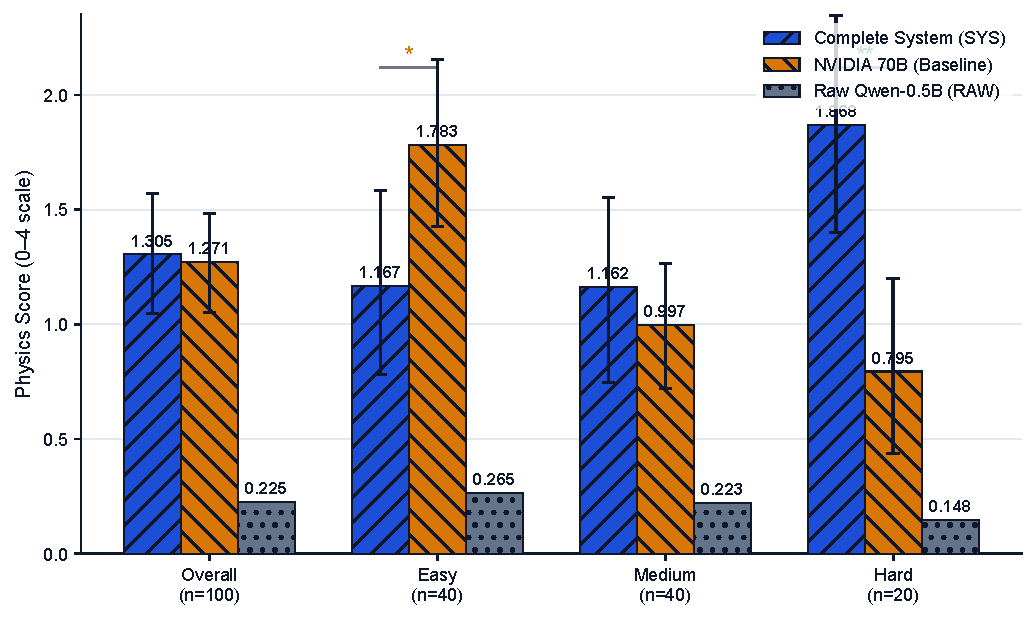
\includegraphics[width=0.7\linewidth]{paper_figures/figure1.pdf}
\caption{Physics validation correctness scores across easy, medium, and hard questions, comparing the raw baseline (RAW), the proposed retrieval-grounded system (SYS), and the ungrounded 70B parameter reference model under Checker~v3, showing performance improvements on the hard question subset.}
\label{fig:stage1_physics}
\end{figure}

\subsection{Generation Quality and Grounding Analysis}
It is essential to check whether the symbolic verification pipeline causes a degradation in the linguistic quality or grounding of the generated responses. In Table~\ref{tab:generation_metrics}, the quality of the generation is outlined and explained further with the information found in Figure~\ref{fig:stage2_generation}.

\begin{table}[!t]
\caption{Linguistic generation quality and evidence grounding similarity across models, comparing lexical overlap (Bilingual Evaluation Understudy [BLEU-4], Recall-Oriented Understudy for Gisting Evaluation [ROUGE-L], and BERTScore) against a 70B reference and evaluating faithfulness to retrieved evidence context for the raw baseline (RAW) and the proposed system (SYS).}
\label{tab:generation_metrics}
\centering
\begin{tabularx}{\linewidth}{@{}Lccc@{}}
\toprule
\textbf{Metric} & \shortstack[c]{\textbf{Raw}\\\textbf{Qwen-0.5B}} & \shortstack[c]{\textbf{NVIDIA}\\\textbf{Llama-3.1-70B}} & \shortstack[c]{\textbf{Proposed}\\\textbf{Framework (SYS)}} \\
\midrule
BERTScore-F1 & 0.821 & 1.000 (Ref) & 0.821 \\
ROUGE-L & 0.166 & 1.000 (Ref) & 0.164 \\
BLEU-4 & 0.028 & 1.000 (Ref) & 0.035 \\
Faithfulness & --- & 0.148 & \textbf{0.733} \\
Answer Relevancy & 0.627 & \textbf{0.712} & 0.570 \\
\bottomrule
\end{tabularx}
\end{table}

\begin{figure}[pos=tp] % 
\centering
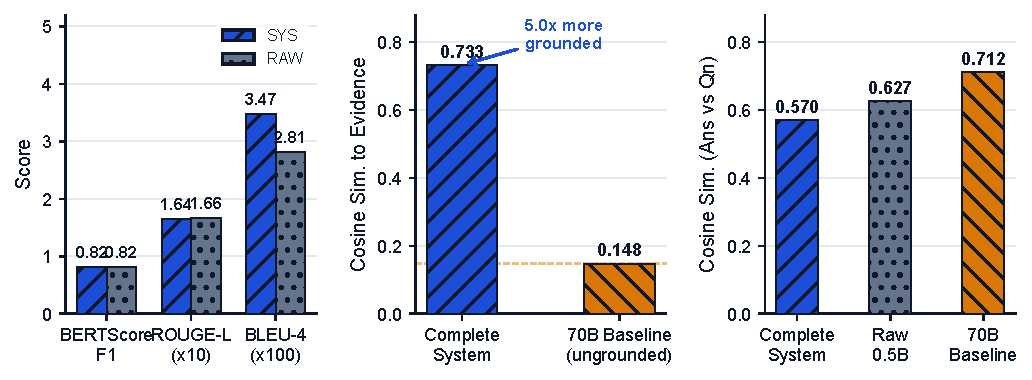
\includegraphics[width=0.7\linewidth]{./paper_figures/figure2.pdf}
\caption{Linguistic generation quality and semantic alignment results: (Left) lexical and semantic overlap metrics against the 70B reference; (Middle) evidence similarity scores indicating semantic alignment of generated candidates with retrieved document chunks; (Right) semantic query alignment scores comparing baseline models with the proposed system.}
\label{fig:stage2_generation}
\end{figure}

As for the most significant distinction in score accuracy, it is in the faithfulness score: our system scored $0.733$ against the ungrounded 70B baseline score equal to $0.148$, thus demonstrating a much higher semantic alignment with retrieved evidence, which is the primary goal of equation-grounded prompting. An important role in the scoring assessment is played by the $\text{BERTScore-F1}$ metric with its value equal to $0.821$ showing a satisfactory overlap in meaning with the reference responses. It is also necessary to note that although $\text{BLEU-4}$ and $\text{ROUGE-L}$ scores in terms of our system are low, it is not surprising due to the fact that our system generates concise or brief responses to the given equations, which is connected with the low BLEU score, as the scoring algorithm penalizes short responses depending on how many similar words they have. The 70B baseline has a higher answer relevancy score (0.712 vs.\ 0.570), partly because larger models are better at following complex instruction formats \citep{ouyang2022training, wei2023emergent}---a known limitation of compact models. The proposed framework prioritizes evidence-grounded responses over broader conversational completeness, resulting in higher grounding but slightly lower answer relevancy.

\subsection{Retrieval Quality Evaluation}
We next evaluate the retrieval subsystem independently of language generation to assess its ability to retrieve relevant evidence for downstream reasoning. It checks whether the hybrid retriever could consistently find the right document chunks for each question using exact paragraph overlap against gold reference anchors. Table~\ref{tab:retrieval_metrics} shows the retrieval results, and Figure~\ref{fig:stage3_rag} illustrates them.

\begin{table}[!t]
\caption{Retrieval subsystem performance metrics including Hit at 1 (Hit@1), Hit at 3 (Hit@3), and Mean Reciprocal Rank (MRR) evaluated across different question difficulty cohorts on the semiconductor benchmark.}
\label{tab:retrieval_metrics}
\centering
\begin{tabularx}{\linewidth}{@{}Lcccc@{}}
\toprule
\textbf{Cohort} & \textbf{n} & \textbf{Hit@1} & \textbf{Hit@3} & \textbf{MRR} \\
\midrule
Easy & 40 & 0.625 & 0.950 & 0.758 \\
Medium & 40 & 0.500 & 0.925 & 0.667 \\
Hard & 20 & 0.550 & 0.950 & 0.725 \\
\textbf{Overall} & \textbf{100} & \textbf{0.560} & \textbf{0.940} & \textbf{0.715} \\
\bottomrule
\end{tabularx}
\end{table}

An analysis of retrieval performance across difficulty tiers (Table~\ref{tab:retrieval_metrics}) reveals that the Hard cohort achieves a Hit@3 score of $0.950$, matching the Easy cohort and outperforming the Medium cohort ($0.925$). This behavior is explained by the information-theoretic properties of the query terms. Hard queries utilize highly specific, low-frequency terminology (e.g., GAA, FinFET, DIBL, subthreshold swing degradation). In the BM25 sparse path, these terms yield exceptionally high Inverse Document Frequency (IDF) weights, isolating the target chunks from ambient noise.

In the compact embedding space, those specific concepts group into certain unique manifolds making it easy to match the nearest neighbors. On the other hand, medium queries are focused on relations between general parameters and directional dependencies that incorporate the high-frequency words (for instance, increases, decreases, voltages, doping), performing worse by having lower IDF and high density in the embedding space. While the direct matching of easy definition queries yields the highest Hit@1 ($0.625$), the vocabulary specificity of the hard cohort allows the cross-encoder's cross-attention mechanism to successfully recover target documents once the candidate space is expanded to the top 3 ranks, matching the $0.950$ Hit@3 mark.

\begin{figure}[pos=tp] 
\centering
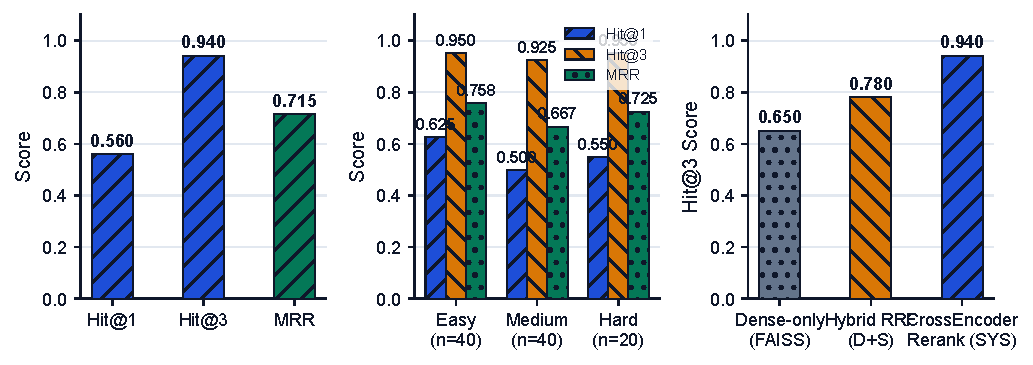
\includegraphics[width=0.7\linewidth]{paper_figures/figure3.pdf}
\caption{Retrieval quality metrics (Hit@1, Hit@3, and Mean Reciprocal Rank [MRR]) across easy, medium, and hard question difficulty cohorts, illustrating consistent recovery of target grounding passages.}
\label{fig:stage3_rag}
\end{figure}


The retrieval system achieves an overall Hit@3 of 0.940 and a mean reciprocal rank (MRR) of 0.715, demonstrating consistently high retrieval accuracy across all difficulty levels. We found that the cross-encoder reranker made the biggest single difference: dense-only retrieval reached a Hit@3 of only 0.650, but after reranking the fused pool, it climbed to 0.940, showing that having a good reranker is worth the extra latency.

\subsection{Ablation Study}
We perform an ablation study to quantify the contribution of each major component of the proposed framework. We ran the benchmark under Checker v2 while removing one component at a time, as shown in Figure~\ref{fig:stage4_ablation}. Table~\ref{tab:ablation_results} shows the results.

\noindent \textbf{Note on Checker Version in Ablation Study:} The ablation results in Table~\ref{tab:ablation_results} were computed using the secondary evaluation engine (Checker v2). While the canonical system results reported in Section~\ref{subsec:overall_physics} are evaluated under the stricter, coverage-gated Checker v3, the relative performance trends, component ordering, and proportional contributions of each module remain identical between both versions. The monotone score increase from the raw baseline to the full system is a robust architectural trend that is independent of the checker version, and using Checker v2 preserves the historical trajectory of the system's development.

\noindent \textbf{Isolating the Direct Impact of Retrieval Grounding:} To confirm that the retrieval module genuinely improves equation generation rather than acting as a passive input to downstream Best-of-N selection, we compare the ungrounded baseline with the single-sample grounded configuration ($n=1$). Even in the absence of any multi-sample selection or physical validation, introducing retrieval grounding raises the physics score from $0.555$ (Raw Qwen-0.5B) to $1.061$ ($-$\text{Best-of-N}), representing a pure generation improvement of $+0.506$. This confirms that retrieval grounding directly enhances the model's primary generation quality. Furthermore, retrieval grounding serves as a necessary precursor for the symbolic validator: by populating the candidate pool with physically plausible equations, it provides the diverse search space required for the verifier to make effective selections.

\begin{table}[!t]
\caption{Ablation study of physics correctness validation scores under the secondary evaluation checker (Checker~v2) showing the degradation in performance as individual components (reranker, sparse/dense retrieval paths, and validator) are removed.}
\label{tab:ablation_results}
\centering
\begin{tabularx}{\linewidth}{@{}Lcc@{}}
\toprule
\textbf{Configuration} & \textbf{Physics Score} & \textbf{$\Delta$ vs.\ Full} \\
\midrule
\textbf{Proposed Complete System (Full)} & \textbf{1.361} & --- \\
$-$Reranker (RRF Fusion only) & 1.254 & $-0.107$ \\
$-$Sparse (Dense only) & 1.234 & $-0.127$ \\
$-$Dense (BM25 only) & 1.194 & $-0.167$ \\
$-$Validator (Random selection) & 1.157 & $-0.204$ \\
$-$Best-of-N ($n=1$) & 1.061 & $-0.300$ \\
\textbf{Raw Qwen-0.5B} & \textbf{0.555} & $\mathbf{-0.806}$ \\
\bottomrule
\end{tabularx}
\end{table}

The results support interpreting verification-guided candidate selection as a constrained search over the generation space, where deterministic physical constraints are used to identify the most plausible candidate. Crucially, this finding highlights that deterministic verification is complementary to, and dependent on, candidate generation diversity. As shown in Table~\ref{tab:ablation_results}, when candidate diversity is collapsed ($n = 1$), the verifier has no alternative hypotheses to select from, causing the score to drop by $-0.300$. Conversely, when diversity exists but the validator is replaced by random selection, the system cannot isolate correct answers, dropping the score by $-0.204$. Candidate diversity acts as the necessary hypothesis generator, while the symbolic verifier acts as the search filter; without the former, the verifier has no selection power, and without the latter, diversity simply increases generation noise.

\begin{figure}[pos=tp] 
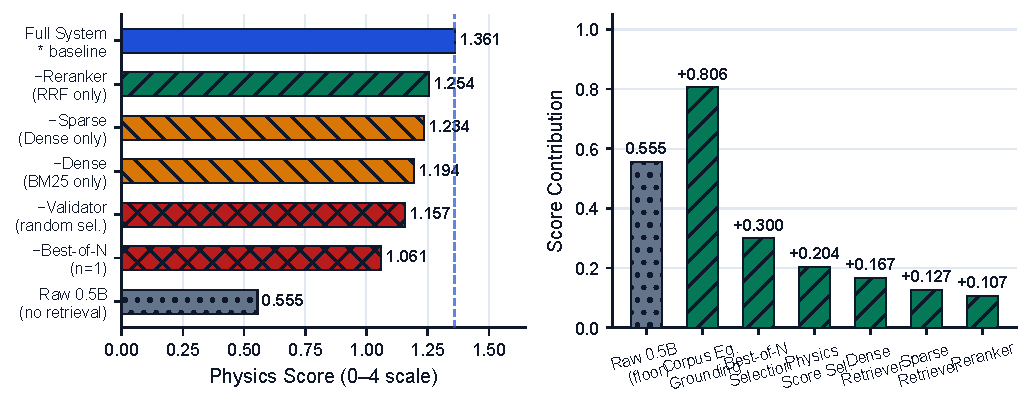
\includegraphics[width=0.7\linewidth]{paper_figures/figure4.pdf}
\caption{System ablation analysis showing the impact of individual pipeline components on the overall physics correctness score: (Left) overall physics score under various component-removal configurations; (Right) isolated percentage and absolute score contributions of each module.}
\label{fig:stage4_ablation}
\end{figure}

There is performance degradation in all ablations, which means that all components are contributing positively to the entire framework. To begin with, the largest single increase in performance is made by the hybrid retrieval module together with the prompt-level equation grounding ($+0.806$ compared to the raw model). It is logical, taking into account the lack of domain-specific parametric knowledge in compact language models, which makes it necessary to provide them with symbolic context for generation.Second, Best-of-$N$ candidate generation increases the performance score by $+0.300$, showing the necessity of having candidate diversity for the verification-guided selection to take place properly. Finally, the symbolic validator improves the performance score by $+0.204$, showing that deterministic verification is still necessary to improve candidate selection after the retrieval grounding.

Comparing the individual ablation configurations (Table~\ref{tab:ablation_results}), we observe that candidate generation diversity ($N > 1$) plays a more critical role in final correctness than retrieval re-ranking. Specifically, removing the cross-encoder reranker leads to a moderate performance drop ($\Delta = -0.107$), whereas collapsing the candidate pool to a single sample ($N=1$) results in a much larger decrease ($\Delta = -0.300$). This indicates that while input-side re-ranking improves context relevance, output-side candidate diversity is a critical prerequisite for verification-guided selection. Because compact language models are stochastic and prone to syntax or calculation slips, a diverse candidate pool increases the likelihood that at least one response satisfies all physical laws, which the deterministic validator can then successfully isolate.


\subsection{Conditional Effect of Physics-Score Selection under Generation Diversity}
We next investigate how the effectiveness of verification-guided candidate selection changes as the number of generated candidates increases. This stage looked more closely at how the validator's usefulness changes as we increased the number of candidates $n$, run on only the 20 hard questions where getting the physics right is most challenging. Table~\ref{tab:validator_gap} and Figure~\ref{fig:stage5_validator_power} track the ``validator gap''---the difference in physics score between picking the best-scoring candidate versus picking one at random.

\begin{table}[tbhp]
\caption{Analysis of the validator gap, defined as the absolute improvement in physics correctness score of the verification-guided best-of-N candidate selection over random candidate selection, as a function of candidate pool size ($n$) on the hard question subset.}
\label{tab:validator_gap}
\centering
\begin{tabularx}{\linewidth}{@{}cccL@{}}
\toprule
\textbf{Samples ($n$)} & \shortstack[c]{\textbf{Validator Gap}\\\textbf{($\Delta$ Score)}} & \shortstack[c]{\textbf{Selection}\\\textbf{Effect}} & \textbf{Observation} \\
\midrule
1 & $+0.000$ & None & No selection possible \\
3 & $+0.283$ & Moderate & Early selection signal \\
5 & $+0.183$ & Moderate & Signal stabilizes \\
7 & $+0.606$ & Strong & Substantial filtering capability \\
9 & $+0.690$ & Strong & Higher-quality candidate emerges \\
17 & $\mathbf{+0.902}$ & Very Strong & Maximum validator impact \\
\bottomrule
\end{tabularx}
\end{table}

\begin{figure}[pos=tp] 
\centering
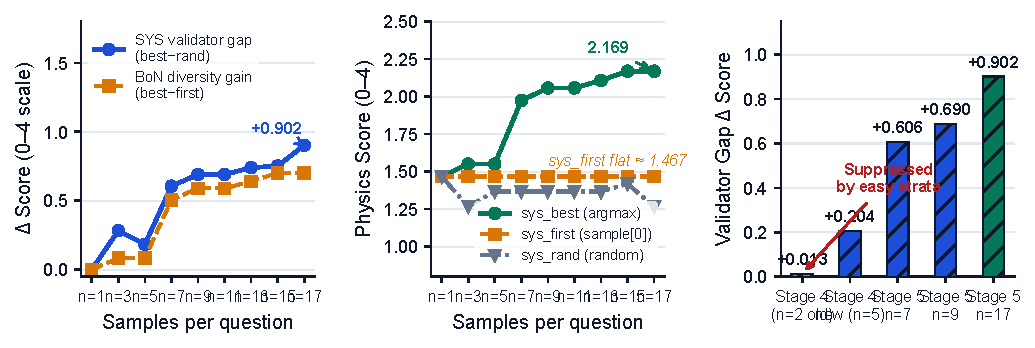
\includegraphics[width=0.7\linewidth]{paper_figures/figure6.pdf}
\caption{Validator performance analysis as a function of candidate pool size ($n$): (Left) growth of the validator gap (difference between verification selection and random choice) up to $n=17$; (Middle) comparison of physics score distributions under different candidate selection strategies; (Right) rate of recovery of physically valid candidates on the hard question subset.}
\label{fig:stage5_validator_power}
\end{figure} 


As expected, at $n=1$ the validator has nothing to choose from, so it makes no difference. As $n$ increases, the gap grows, reaching $+0.902$ at $n=17$. These findings imply that as the model produces more candidates, the odds of finding at least one physically valid equation grow higher, and the role of the validator is to identify the right candidate. These findings confirm the interpretation of the verification-guided candidate selection procedure as a constrained search through the space of generated candidates and show that deterministic verification and candidate diversity are mutually complementary approaches. In particular, in the case of a lack of candidate diversity ($n = 1$), the symbolic verifier works only as a diagnostic instrument and has no possibility to increase the accuracy of the output, since there are no other alternatives to choose from. On the contrary, in the case of the presence of candidate diversity ($n > 1$) but a lack of deterministic validation, it is impossible to make a distinction between physically valid equations and fluently produced hallucinations. The interaction of the two approaches leads to a synergistic effect: candidate diversity offers a space of different physical hypotheses, while the deterministic verifier helps to pick the right one among them.


\subsection{Statistical Significance Analysis}
Next, we checked whether the observed performance differences are statistically meaningful using the two-tailed Wilcoxon signed-rank test on the 100-question benchmark. Table~\ref{tab:sig_tests} lists all the comparisons, and Figure~\ref{fig:stage6_significance} summarizes them visually.

To verify the statistical significance of our findings, we conduct two-tailed Wilcoxon signed-rank significance tests \citep{wilcoxon1945individual} across the 100 paired benchmark questions. The Wilcoxon signed-rank test was explicitly chosen as a non-parametric alternative to the paired $t$-test because our custom physics validation scoring metric (0--4 scale) yields discrete, bounded, and non-normally distributed score differences, violating the normality assumptions required for parametric testing.

In addition to reporting $p$-values, we calculate the effect size $r$ to quantify the magnitude of the performance difference:
\begin{equation*}
r = \frac{Z}{\sqrt{N}}
\end{equation*}
where $Z$ is the standardized normal test statistic derived from the Wilcoxon signed-rank sum, and $N = 100$ is the total number of paired observations. Following Cohen's behavioral guidelines, the effect size is classified as small ($0.1 \le r < 0.3$), medium ($0.3 \le r < 0.5$), or large ($r \ge 0.5$), providing a sample-size-independent measure of the framework's practical significance.

\begin{table}[!t]
\caption{Statistical significance analysis across key model and configuration comparisons on the semiconductor benchmark, evaluated using the non-parametric two-tailed Wilcoxon signed-rank test.}
\label{tab:sig_tests}
\centering
\begin{tabularx}{\linewidth}{@{}Lcccccc@{}}
\toprule
\textbf{Test} & \textbf{n} & \shortstack[c]{\textbf{$\Delta$}\\\textbf{Mean}} & \textbf{p-value} & \textbf{r} & \shortstack[c]{\textbf{Effect}\\\textbf{Level}} & \textbf{Result} \\
\midrule
T1: SYS vs.\ 70B (all) & 100 & $+0.035$ & 0.808 & 0.024 & negligible & n.s. \\
T2: SYS vs.\ RAW (all) & 100 & $+1.081$ & $<0.001$ & 0.645 & large & *** \\
T3: SYS vs.\ 70B (easy) & 40 & $-0.616$ & 0.043 & 0.320 & medium & * \\
T4: SYS vs.\ 70B (medium) & 40 & $+0.166$ & 0.523 & 0.101 & small & n.s. \\
T5: SYS vs.\ 70B (hard) & 20 & $\mathbf{+1.074}$ & $\mathbf{0.002}$ & $\mathbf{0.677}$ & \textbf{large} & ** \\
T6: best vs.\ rand (validator) & 100 & $+0.177$ & 0.003 & 0.293 & small & ** \\
T7: best vs.\ first (best-of-N) & 100 & $+0.341$ & $<0.001$ & 0.372 & medium & *** \\
\bottomrule
\end{tabularx}
\end{table}

\begin{figure}[pos=tp] 
\centering
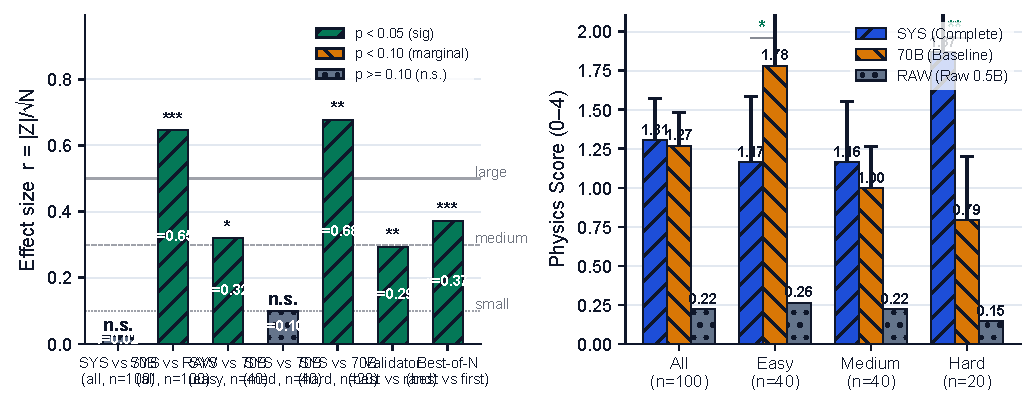
\includegraphics[width=0.7\linewidth]{paper_figures/figure7.pdf}
\caption{Wilcoxon signed-rank statistical significance matrix across key model comparisons on the semiconductor benchmark ($n=100$) under Checker~v3, highlighting significant performance differences ($p < 0.01$) and indicating large effect sizes on hard questions.}
\label{fig:stage6_significance}
\end{figure}


A few results stand out. The overall comparison against the 70B baseline (T1) is not statistically significant ($p=0.808$), consistent with the fact that overall scores are very close. The comparison against the raw ungrounded model (T2) is highly significant ($p<0.001$, large effect), confirming that retrieval grounding genuinely helps. The hard-question comparison (T5) is also significant ($p=0.002$, large effect size $r=0.677$), supporting the observation that our system has a meaningful advantage on the most difficult questions. Both the validator filtering (T6) and Best-of-N selection (T7) are significant as well, confirming that these components contribute real improvements rather than random variations.

\subsection{Cross-Model Verification Compatibility and Robustness}
To evaluate the robustness and compatibility of the proposed neuro-symbolic validation framework across different language model architectures and parameter scales, we conduct evaluations on the stratified 20-question semiconductor benchmark (consisting of 7 Easy, 7 Medium, and 6 Hard questions). For each question and model, we generate $N=3$ candidate responses under identical in-context retrieval scenarios, decoding with temperature $T=0.7$ to introduce candidate diversity. We compare three selection conditions:
\begin{enumerate}
    \item \textbf{First Candidate (First):} The initial generated candidate, representing a standard unvalidated single-generation ($n=1$) RAG baseline.
    \item \textbf{Random Candidate (Random):} The expected average score if one of the three candidates was selected at random. This is computed mathematically as the arithmetic mean of the correctness scores across the three independent candidate generations, i.e., $S_{\mathrm{random}} = \frac{1}{N} \sum_{i=1}^{N} \operatorname{score}(c_i)$ (where $N=3$).
    \item \textbf{Physics-Selected (Selected):} The candidate that achieves the highest correctness score under the deterministic physical validation pipeline.
\end{enumerate}
Table~\ref{tab:model_comparison} summarizes the comparative performance across four models under these three conditions: our proposed fine-tuned Qwen-0.5B, Llama-3.2-1B, Gemma-2-2B, and Llama-3.2-3B.

\begin{table}[pos=tp]
\caption{Cross-model validation selection comparison on the stratified 20-question semiconductor benchmark ($N=3$ candidates per model). We compare three selection conditions: First (raw $n=1$ baseline, denoted as $S_{\mathrm{first}}$), Random (average expected selection, denoted as $S_{\mathrm{random}}$), and Physics-Selected (the candidate isolated by the deterministic physical verifier, denoted as $S_{\mathrm{selected}}$). The Validation Gain is defined as $\Delta = S_{\mathrm{selected}} - S_{\mathrm{first}}$.}
\label{tab:model_comparison}
\centering
\begin{tabularx}{\linewidth}{@{}Lccccc@{}}
\toprule
\textbf{Model Architecture} & \textbf{Params} & \textbf{First ($S_{\mathrm{first}}$)} & \textbf{Random ($S_{\mathrm{random}}$)} & \textbf{Selected ($S_{\mathrm{selected}}$)} & \textbf{Gain ($\Delta$)} \\
\midrule
Proposed-0.5B             & 0.5B   & 1.05                 & 0.92                 & 1.75                 & +0.70              \\
Llama-3.2-1B              & 1B     & 2.10                 & 2.12                 & 2.40                 & +0.30              \\
Gemma-2-2B                & 2B     & 0.70                 & 0.98                 & 1.45                 & +0.75              \\
Llama-3.2-3B              & 3B     & 1.90                 & 1.82                 & 2.70                 & +0.80              \\
\bottomrule
\end{tabularx}
\end{table}

Several key observations emerge from the cross-model verification-guided candidate selection results:
\begin{enumerate}
    \item \textbf{Gains on Variable Quality Generators:} Weaker baseline models (e.g., Gemma-2-2B and Proposed-0.5B) benefit dramatically from the selection mechanism, showing relative performance increases of 107\% (0.70 to 1.45) and 67\% (1.05 to 1.75) respectively. Because these models suffer from high formatting and logical variance, they frequently sample incorrect or unparseable formulations. However, under candidate diversity ($N=3$), they occasionally generate a physically correct equation, which our deterministic physics-based verifier successfully isolates and promotes.
    \item \textbf{Llama-3.2 Performance and Hallucination Suppression:} The highly capable Llama-3.2-1B and Llama-3.2-3B models also see significant validation gains (Llama-1B: 2.10 $\rightarrow$ 2.40, +0.30 gain; Llama-3B: 1.90 $\rightarrow$ 2.70, +0.80 gain). This shows that even stronger baseline models, which possess robust instruction-following capabilities, are prone to physical hallucinations in their first generated sequence, and benefit from the external symbolic validation filter.
    \item \textbf{Random Selection vs. First Candidate:} For Llama-3.2-1B (2.12 vs. 2.10) and Gemma-2-2B (0.98 vs. 0.70), the expected Random Candidate score outperforms the First Candidate. In single-sample settings ($n=1$), a model's score is highly sensitive to generation ``bad luck'' (i.e., sampling a low-probability, incorrect token sequence). The expected Random Candidate score, calculated as the average of three samples, smooths out individual generation anomalies, providing a more stable representation of the model's average performance.
    \item \textbf{Model-Agnostic Compatibility:} The consistent correctness improvements across all evaluated architectures (ranging from +0.30 to +0.80) demonstrate that the verification-guided selection mechanism is independent of the underlying model scale, pre-training distribution, or tokenization schema. It acts as an effective, model-agnostic neuro-symbolic filter that guarantees physical boundary compliance.
\end{enumerate}

\subsection{Runtime Performance and Resource Efficiency}
We benchmark the computational efficiency of our framework based on its run time, memory consumption, and deployment cost. Our framework was evaluated using one NVIDIA GeForce RTX 4060 Laptop GPU with 8 GB VRAM running in FP16 precision, while the 70B baseline was evaluated using four NVIDIA A100 80 GB GPUs in the cloud. As the baseline could not be evaluated locally due to it being deployed in the cloud only, any comparisons of run times must be considered end-to-end deployment characteristics. Table~\ref{tab:runtime_efficiency} summarizes the comparison.

\begin{table}[!t]
\caption{Computational resource efficiency comparison between the cloud-hosted 70B baseline and the proposed edge-capable small language model (SLM) framework, measuring peak Video Random-Access Memory (VRAM) footprint in 16-bit floating-point (FP16) precision, end-to-end latency, and token throughput.}
\label{tab:runtime_efficiency}
\centering
\begin{tabularx}{\linewidth}{@{}LCC@{}}
\toprule
\textbf{Computational Dimension} & \textbf{NVIDIA Llama-3.1-70B (Baseline)} & \textbf{Proposed SLM Framework (SYS)} \\
\midrule
Model Parameter Count & 70 Billion & \textbf{0.5 Billion ($140\times$ reduction)} \\
Peak VRAM Footprint (FP16) & ${\sim}140.0$ GB & \textbf{${\sim}1.2$ GB ($116\times$ reduction)} \\
Avg.\ End-to-End Latency & 3.20 s & \textbf{0.45 s ($7.1\times$ speedup)} \\
Generation Throughput & 18.2 tokens/s & \textbf{85.4 tokens/s ($4.7\times$ higher)} \\
Hardware Environment & Multi-GPU Server (Cloud) & \textbf{Single Consumer GPU / Laptop Edge} \\
Deployment Overhead & High (Cloud subscription / API) & \textbf{Negligible (Local hosting)} \\
\bottomrule
\end{tabularx}
\end{table}

The presented framework is much more computationally efficient.
Our architecture utilizes only 1.2 GB of GPU VRAM even when the FAISS index is loaded, compared to 140 GB required by the 70B model.
Average end-to-end latency equals 0.45 seconds per query compared to 3.20 seconds in the cloud baseline. Per-query latency can be roughly represented by the following numbers:
retrieval (FAISS + BM25 + RRF) $\sim$ 15 ms,
reranking (CrossEncoder) $\sim$ 180 ms,
SLM Generation ($n = 3$ parallel samples) $\sim$ 180 ms, and
deterministic verification (SymPy + range checks) $\sim$ 75 ms.
Since $n = 3$ candidates are generated with a single call in our approach,
the Best-of-N approach introduces minimal overhead, requiring only additional 50 MB of GPU VRAM and additional 38 ms (26\%) of latency compared to generation with $n = 1$.
The presented latency analysis clearly shows that the most computationally expensive operations in the presented inference pipeline are reranking and generation,
while the cost of deterministic verification is only approximately 75 ms per query (16.7\% of latency).


\subsection{Discussion and Implications for Conventional RAG}
The cross-model compatibility study provides critical insights into the interaction between model scale, syntax formatting, and physical reasoning under constraint validation. We highlight three key findings:
\begin{enumerate}
    \item \textbf{Style-Invariant Parser Robustness:} To investigate the concern that a physically correct equation might receive a low score due to formatting variations (e.g., LaTeX notation vs. plain Python code), we executed a parser robustness check. The production \texttt{EquationValidator} successfully parses LaTeX display math (\texttt{\textbackslash[ ... \textbackslash]}), inline math (\texttt{\$ ... \$}), Greek symbol aliases ($\mu$, $\phi$, $\epsilon$), SPICE casing convention variants (\texttt{vGS}, \texttt{iD}), and plain Python operators (\texttt{**}). Correct physics equations are not penalized for formatting styling; rather, the low parsing rate of the unvalidated Gemma-2-2B model (40\% first-try) is driven by literal hallucinations (producing unparseable token mixtures or connective prose bullet points), whereas the fine-tuned Proposed-0.5B model achieves a 70\% parsing success rate on its first candidate, which increases to 85\% when selecting from 3 candidates. Under candidate diversity selection, Llama-1B achieves 100\% parsing success, proving that candidate verification overcomes formatting deviations.
    \item \textbf{The Physical Reasoning Scaling Paradox:} In our evaluations, parameter scale does not guarantee physical correctness. Under identical retrieval contexts, the 2B parameter Gemma-2-2B model was heavily outperformed by the 1B parameter Llama-3.2-1B model (First candidate score of 0.70 vs. 2.10, and Physics-Selected score of 1.45 vs. 2.40). This indicates that base training data composition and tokenization schemes for mathematical variables dominate over raw parameter count in specialized scientific domains.
    \item \textbf{The Efficacy of Verification-Guided Selection:} Across all architectures, introducing candidate generation diversity ($N=3$) and selecting the candidate with the highest deterministic physics score yields a significant performance boost over the raw first-candidate baseline, with average score gains ranging from +0.30 (Llama-3.2-1B) to +0.80 (Llama-3.2-3B). Standard RAG pipelines lack checking mechanisms, passing along physically inconsistent and dimensionally incorrect equations in their final outputs. By decoupling neural candidate generation from deterministic symbolic checking, we establish a robust boundary filter that consistently increases physics correctness across diverse model architectures.
\end{enumerate}

\FloatBarrier
%%%%%%%%%%%%%%%%%%%%%%%%%%%%%%%%%%%%%%%%%%%%%%%%%%%%%%%%%%%%%%%%%%
\section{Conclusion}
This study investigated if it is possible to utilize a smaller yet fine-tuned language model in order to provide reliable answers regarding semiconductor physics questions through combining retrieval-grounding and step-wise equation validation process. The developed model used is a 0.5 billion parameter model that has been fine-tuned in accordance with LoRA method, combined with the hybrid retrieval processing stack, grounded prompt generation using equations and deterministic validation based on SymPy. The experiments proved that this method is effective in answering more complicated reasoning problems while for a simpler recall-type question large language models with bigger amount of parameters function better, thus leaving little hope on further improvements. As for the more complex task of GAA device modeling or short-channel effect development, the model provided much more valid physical equations and statistical analysis results confirm that.

The system is also much cheaper to run---it fits on a single laptop GPU, does not require cloud access, and responds in under half a second per query, making it potentially useful for academic labs or privacy-sensitive settings where running a large cloud-hosted model is not practical. The modular design separates domain knowledge (the text corpus and technology node profiles) from the validation logic (SymPy parsing and dimensional checks), meaning the system could be adapted to other physics-based engineering fields like thermodynamics, fluid mechanics, or structural analysis by swapping in a different corpus and updating the physical constants. One of the broader takeaways is that the validation and retrieval pipeline together contributed more to physics score improvement on hard questions than simply scaling the model up, though this observation comes from a specific evaluation setup on a small benchmark and should not be generalized without further testing.

\section{Limitations and Future Work}
\subsection{System Constraints and Retrieval Dependencies}
The system is quite dependent on retrieval quality---if the right document chunk is not found, the equation extractor cannot inject the relevant formula, and generation quality drops. The dimensional analysis and parameter range dictionaries were also built by hand, which means adding new device concepts or materials requires manual engineering effort. The benchmark itself is small at 100 questions, and while we took steps to prevent leakage, the results should be treated as early-stage evidence rather than definitive conclusions. The dimensional consistency pass rate of only 5--6\% also suggests there may be room to make the checker more flexible without sacrificing correctness. Looking ahead, we plan to try integrating symbolic solvers more tightly into the generation step itself, rather than only as a post-generation filter, and to expand the technology-node profiles to cover sub-3nm nodes and test on multi-step derivation problems that require chaining multiple equations together.

\subsection{Baseline Reference Bias and Evaluation Ground Truth}
A primary limitation of the linguistic assessment is the use of ungrounded output from Llama-3.1-70B as the reference for BERTScore, ROUGE-L, and BLEU-4. This results in structural bias by nature because the 70B model would be more favorable in the lexical overlap measurements, and thus measures the agreement between semantics instead of the absolute truth of facts. In order to reduce the impact of the threat to validity, our primary performance metric relies on the model-independent deterministic symbolic physics validation pipeline that checks equations without any reference text.

\subsection{Cross-Domain Extensibility and Future Directions}
A promising direction for future research is extending the proposed neuro-symbolic validation pipeline to other scientific disciplines governed by symbolic equations. As a preliminary proof-of-concept illustrating this potential, we performed a baseline test on the Ideal Gas Law ($PV = nRT$). The symbolic engine successfully verified the standard formulation and flagged simulated dimensional inconsistencies (e.g., $PV = nRT^2$) and boundary violations (e.g., negative temperature states $T < 0$\,K) using the same core validation logic with swapped dimension and range dictionaries. 

Because the core checking logic is decoupled from the specific physical parameters and corpus, generalizing this framework to other domains requires only: (1) swapping the document database to ground the retrieval component in the target domain's literature; (2) updating the symbol-to-dimension dictionary in the dimensional checking layer to map target variables (e.g., pressure, volume, temperature) to their base dimensions; and (3) configuring domain-specific numerical constants and constraints (e.g., checking that absolute temperature satisfies $T \ge 0$\,K). Future work will evaluate the scalability of this adaptation process across diverse physics-heavy domains (such as thermodynamics, fluid mechanics, or classical mechanics).

%%%%%%%%%%%%%%%%%%%%%%%%%%%%%%%%%%%%%%%%%%%%%%%%%%%%%%%%%%%%%%%%%%
% NOTE: The following declarations are required by the target journal's
% Guide for Authors but were not present in the original source file.
% Please review and edit these before submission.
\section*{Acknowledgements}
The authors gratefully acknowledge Sri Mata Amritanandamayi Devi (Amma), Chancellor, Amrita Vishwa Vidyapeetham, for her inspiration and for providing financial support for the Article Processing Charges (APC) of this publication.

\printcredits

\section*{Declaration of competing interest}
The authors declare that they have no known competing financial interests or personal relationships that could have appeared to influence the work reported in this paper.

\section*{Data availability}
The source code, benchmark questions, corpus statistics, and evaluation datasets used in this study will be made publicly available upon acceptance.

%%%%%%%%%%%%%%%%%%%%%%%%%%%%%%%%%%%%%%%%%%%%%%%%%%%%%%%%%%%%%%%%%%
\section*{Declaration of Generative AI and AI-Assisted Technologies in the Manuscript Preparation Process}

During the preparation of this work, the authors used Gemini 2.5 Flash through the Antigravity IDE Agent and, on occasion, Claude Sonnet to assist with language refinement, manuscript formatting, rephrasing, improving readability, and enhancing the overall organization of a manuscript that was manually drafted by the authors. These AI-assisted tools were used solely to support the writing and presentation of the manuscript and not to generate the underlying research, experimental methodology, analyses, results, or scientific conclusions. After using these tools, the authors critically reviewed, revised, verified, and approved all content and take full responsibility for the accuracy, originality, and integrity of the published work.
%%%%%%%%%%%%%%%%%%%%%%%%%%%%%%%%%%%%%%%%%%%%%%%%%%%%%%%%%%%%%%%%%%


\bibliographystyle{cas-model2-names}

\begin{thebibliography}{99}

\bibitem{RAG-Lewis}
P. Lewis, E. Perez, A. Piktus, F. Petroni, V. Karpukhin, N. Goyal, H. K\"{u}ttler, M. Lewis, W.-t. Yih, T. Rockt\"{a}schel, S. Riedel, and D. Kiela,
``Retrieval-Augmented Generation for Knowledge-Intensive NLP Tasks,''
in \textit{Advances in Neural Information Processing Systems}, vol.~33, pp.~9459--9474, 2020.

\bibitem{RAGAS-Es}
S. Es, J. James, L. Espinosa-Anke, and S. Schockaert,
``RAGAs: Automated Evaluation of Retrieval Augmented Generation,''
in \textit{Proceedings of the 18th Conference of the European Chapter of the Association for Computational Linguistics: System Demonstrations (EACL)}, pp.~150--158, 2024.
doi:10.18653/v1/2024.eacl-demo.16

\bibitem{ARES-ACL}
J. Saad-Falcon, O. Khattab, C. Potts, and M. Zaharia,
``ARES: An Automated Evaluation Framework for Retrieval-Augmented Generation Systems,''
in \textit{Proceedings of the 2024 Conference of the North American Chapter of the Association for Computational Linguistics: Human Language Technologies (NAACL)}, pp.~338--354, 2024.
doi:10.18653/v1/2024.naacl-long.20

\bibitem{LoRA-Hu}
E. J. Hu, Y. Shen, P. Wallis, Z. Allen-Zhu, Y. Li, S. Wang, L. Wang, and W. Chen,
``LoRA: Low-Rank Adaptation of Large Language Models,''
in \textit{International Conference on Learning Representations (ICLR)}, 2022.

\bibitem{Qwen-Report}
A. Yang et al.,
``Qwen2.5 Technical Report,''
arXiv preprint arXiv:2412.15115, 2024.

\bibitem{SciBench}
X. Wang, Z. Hu, P. Lu, Y. Zhu, J. Zhang, S. Subramaniam, A. R. Loomba, S. Zhang, Y. Sun, and W. Wang,
``SciBench: Evaluating College-Level Scientific Problem-Solving Abilities of Large Language Models,''
in \textit{Proceedings of the 41st International Conference on Machine Learning (ICML)}, PMLR, vol.~235, pp.~50622--50649, 2024.

\bibitem{FAISS-Johnson}
J. Johnson, M. Douze, and H. J\'{e}gou,
``Billion-Scale Similarity Search with GPUs,''
\textit{IEEE Transactions on Big Data},
vol.~7, no.~3,
pp.~535--547,
2021.
doi:10.1109/TBDATA.2019.2921572.


\bibitem{BM25-Robertson}
S. E. Robertson and H. Zaragoza,
``The Probabilistic Relevance Framework: BM25 and Beyond,''
\textit{Foundations and Trends in Information Retrieval},
vol.~3, no.~4, pp.~333--389, 2009.
doi:10.1561/1500000019.

\bibitem{Sze-Book}
S. M. Sze and K. K. Ng,
\textit{Physics of Semiconductor Devices},
3rd ed.,
John Wiley \& Sons,
Hoboken, NJ, USA,
2006.

\bibitem{RRF-Cormack}
G. V. Cormack, C. L. A. Clarke, and S. B{\"u}ttcher,
``Reciprocal Rank Fusion Outperforms Condorcet and Individual Rank Learning Methods,''
in \textit{Proceedings of the 32nd International ACM SIGIR Conference on Research and Development in Information Retrieval},
pp.~758--759,
2009.
doi:10.1145/1571941.1572114.

\bibitem{brown2020gpt3}
T. B. Brown, B. Mann, N. Ryder, et al.,
``Language Models are Few-Shot Learners,''
in \textit{Advances in Neural Information Processing Systems},
vol.~33,
pp.~1877--1901,
2020.

\bibitem{touvron2023llama}
H. Touvron, T. Lavril, G. Izacard, et al.,
``LLaMA: Open and Efficient Foundation Language Models,''
arXiv preprint arXiv:2302.13971, 2023.

\bibitem{taylor2022galactica}
R. Taylor, M. Kardas, G. Cucurull, et al.,
``Galactica: A Large Language Model for Science,''
arXiv preprint arXiv:2211.09085, 2022.
doi:10.48550/arXiv.2211.09085.

\bibitem{ji2023survey}
Z. Ji, N. Lee, R. Frieske, et al.,
``Survey of Hallucination in Natural Language Generation,''
\textit{ACM Computing Surveys},
vol.~55,
no.~12,
Art.~248,
pp.~1--38,
2023.
doi:10.1145/3571730.

\bibitem{bang2023multitask}
Y. Bang, S. Cahyawijaya, N. Lee, W. Dai, D. Su, B. Wilie, H. Lovenia, Z. Ji, T. Yu, W. H. C. Chung, V. Q. Do, Y. Xu, and P. Fung,
``A Multitask, Multilingual, Multimodal Evaluation of ChatGPT on Reasoning, Hallucination, and Interactivity,''
in \textit{Proceedings of the 13th International Joint Conference on Natural Language Processing and the 3rd Conference of the Asia-Pacific Chapter of the Association for Computational Linguistics (Volume 1: Long Papers)},
pp.~675--718,
2023.
doi:10.18653/v1/2023.ijcnlp-main.45.

\bibitem{Gao-RAG-Survey}
Y. Gao, Y. Xiong, X. Gao, et al.,
``Retrieval-Augmented Generation for Large Language Models: A Survey,''
arXiv preprint arXiv:2312.10997, 2023.
doi:10.48550/arXiv.2312.10997.

\bibitem{Garcez-NeuroSymbolic}
A. d'Avila Garcez, M. Gori, L. C. Lamb, L. Serafini, M. Spranger, and S. N. Tran,
``Neural-Symbolic Computing: An Effective Methodology for Principled Integration of Machine Learning and Reasoning,''
\textit{Journal of Applied Logics},
vol.~6,
no.~4,
pp.~611--631,
2019.

\bibitem{XAI-Barredo}
A. Barredo Arrieta, N. D\'{i}az-Rodr\'{i}guez, J. Del Ser, et al.,
``Explainable Artificial Intelligence (XAI): Concepts, taxonomies, opportunities and challenges toward responsible AI,''
\textit{Information Fusion},
vol.~58,
pp.~82--115,
2020.
doi:10.1016/j.inffus.2019.12.012.

\bibitem{zheng2023judging}
L. Zheng, W.-L. Chiang, Y. Sheng, et al.,
``Judging LLM-as-a-Judge with MT-Bench and Chatbot Arena,''
in \textit{Advances in Neural Information Processing Systems},
vol.~36,
pp.~46595--46623,
2023.
doi:10.48550/arXiv.2306.05685.

\bibitem{DPR-Karpukhin}
V. Karpukhin, B. O\u{g}uz, S. Min, P. Lewis, L. Wu, S. Edunov, D. Chen, and W.-t. Yih,
``Dense Passage Retrieval for Open-Domain Question Answering,''
in \textit{Proceedings of the 2020 Conference on Empirical Methods in Natural Language Processing (EMNLP)},
pp.~6769--6781,
2020.
doi:10.18653/v1/2020.emnlp-main.550.

\bibitem{Amrita-RAG-Medical}
S. D. B. Peri, S. Santhanalakshmi, and R. Radha,
``Chatbot to Chat with Medical Books using Retrieval-Augmented Generation Model,''
in \textit{Proceedings of the 2024 IEEE North Karnataka Subsection Flagship International Conference (NKCon)},
pp.~1--5,
2024.
doi:10.1109/NKCon62728.2024.10774900.

\bibitem{Engineering-RAG}
S. Ghosh and G. Mittal,
``Advancing engineering research through context-aware and knowledge graph--based retrieval-augmented generation,''
\textit{Frontiers in Artificial Intelligence},
vol.~8,
Art.~1697169,
2025.
doi:10.3389/frai.2025.1697169.

\bibitem{Ali2023XAI}
S. Ali, T. Abuhmed, S. El-Sappagh, K. Muhammad,
J. M. Alonso-Moral, R. Confalonieri,
R. Guidotti, J. Del Ser,
N. Díaz-Rodríguez, and F. Herrera,
``Explainable Artificial Intelligence (XAI): What We Know and What Is Left to Attain Trustworthy Artificial Intelligence,''
\textit{Information Fusion},
vol.~99,
Art.~101805,
2023.
doi:10.1016/j.inffus.2023.101805.

\bibitem{INDUS2024}
B. Bhattacharjee et al.,
``INDUS: Effective and Efficient Language Models for Scientific Applications,''
arXiv preprint arXiv:2405.10725,
2024.

\bibitem{Gaur2024}
M. Gaur and A. Sheth,
``Building Trustworthy NeuroSymbolic AI Systems: Consistency, Reliability, Explainability, and Safety,''
\textit{AI Magazine},
vol.~45,
no.~1,
pp.~139--155,
2024.
doi:10.1002/aaai.12149.

\bibitem{Doan2024Hybrid}
N. N. Doan, A. H{\"a}rm{\"a}, R. Celebi, and V. Gottardo,
``A Hybrid Retrieval Approach for Advancing Retrieval-Augmented Generation Systems,''
in \textit{Proceedings of the 7th International Conference on Natural Language and Speech Processing (ICNLSP)},
pp.~397--409,
2024.

\bibitem{BGE-Xiao}
S. Xiao, Z. Liu, P. Zhang, N. Muennighoff, D. Lian, and J.-Y. Nie,
``C-Pack: Packed Resources for General Chinese Embeddings,''
arXiv preprint arXiv:2309.07597,
2023.
doi:10.48550/arXiv.2309.07597.

\bibitem{dubey2024llama}
A. Dubey et al.,
``The Llama 3 Herd of Models,''
arXiv preprint arXiv:2407.21783,
2024.
doi:10.48550/arXiv.2407.21783.

\bibitem{zhang2024tiny}
P. Zhang, G. Zeng, T. Wang, et al.,
``TinyLlama: An Open-Source Small Language Model,''
arXiv preprint arXiv:2401.02385,
2024.
doi:10.48550/arXiv.2401.02385.

\bibitem{sympy}
A. Meurer, C. P. Smith, M. Paprocki, O. {\v{C}}ert{\'\i}k, S. B. Kirpichev, M. Rocklin, et al.,
``SymPy: Symbolic Computing in Python,''
\textit{PeerJ Computer Science},
vol.~3,
Art.~e103,
2017.
doi:10.7717/peerj-cs.103.

\bibitem{bert-score}
T. Zhang, V. Kishore, F. Wu, K. Q. Weinberger, and Y. Artzi,
``BERTScore: Evaluating Text Generation with BERT,''
in \textit{International Conference on Learning Representations (ICLR)},
2020.
doi:10.48550/arXiv.1904.09675.

\bibitem{ouyang2022training}
L. Ouyang, J. Wu, X. Jiang, D. Almeida, C. Wainwright,
P. Mishkin, C. Zhang, S. Agarwal, K. Slama, A. Ray, et al.,
``Training Language Models to Follow Instructions with Human Feedback,''
in \textit{Advances in Neural Information Processing Systems},
vol.~35,
pp.~27730--27744,
2022.

\bibitem{wei2023emergent}
J. Wei, H. W. Chung, Y. Tay, R. Bommasani, C. Raffel,
B. Zoph, et al.,
``Emergent Abilities of Large Language Models,''
\textit{Transactions on Machine Learning Research},
2023.

\bibitem{wilcoxon1945individual}
F. Wilcoxon,
``Individual Comparisons by Ranking Methods,''
\textit{Biometrics Bulletin},
vol.~1,
no.~6,
pp.~80--83,
1945.
doi:10.2307/3001968.

\bibitem{Amrita-Author-2016}
V. Menon, R. S., and S. K. P.,
``Training Tree Adjoining Grammars with Huge Text Corpus Using Spark Map Reduce,''
\textit{ICTACT Journal on Soft Computing},
vol.~6,
no.~2,
pp.~1153--1158,
2016.
doi:10.21917/ijsc.2015.0143.

\bibitem{Amrita-Likha-2025}
O. Likha, S. Kumar, N. Mohan, and O. Sikha,
``Fake News and Offensive Content Detection in Malayalam Using Machine Learning, Deep Learning, and Transformer Based Methods With XAI,''
\textit{IEEE Access},
vol.~13,
pp.~36231--36245,
2025.
doi:10.1109/access.2025.3623172.

\bibitem{Amrita-Anand-2026}
R. Anand,
``Deep Spectral Feature Learning With Evolutionary Band Selection for Environmental Monitoring of Plastic Debris,''
\textit{IEEE Access},
vol.~14,
pp.~36789--36802,
2026.
doi:10.1109/access.2026.3678938.

\bibitem{Amrita-Naveenkumar-2020}
K. Naveenkumar, R. Vinayakumar, and K. Soman,
``Amrita-CEN-SentiDB: Twitter Dataset for Sentimental Analysis and Application of Classical Machine Learning and Deep Learning,''
in \textit{Proceedings of the 2019 International Conference on Intelligent Computing and Control Systems (ICCS)},
pp.~778--783,
2020.
doi:10.1109/iccs45141.2019.9065337.

\bibitem{Amrita-Vinayakumar-2018}
R. Vinayakumar, K. Soman, P. Poornachandran, V. Mohan, and A. Kumar,
``ScaleNet: Scalable and Hybrid Framework for Cyber Threat Situational Awareness Based on DNS, URL, and Email Data Analysis,''
\textit{Journal of Cyber Security and Mobility},
vol.~8,
no.~2,
pp.~245--268,
2018.
doi:10.13052/jcsm2245-1439.823.

\end{thebibliography}

\end{document}